% Ricerca su Wallis e Lipari
% Template usato: Stylish Article 2.2, LaTeX Template.
% Licenza: CC BY-NC_SA 3.0 (https://creativecommons.org/licenses/by-nc-sa/3.0/)

% Librerie Usate
\PassOptionsToPackage{dvipsnames}{xcolor}
\documentclass[fleqn,11pt]{SelfArx} % Template 

\usepackage[italian]{babel} 
\usepackage{pgfplots}
\usepackage{siunitx}
\usepackage{eurosym}
\usepackage{float}
\usepackage{tikz}
\usepackage{parskip}
\usepackage{enumitem}
\usepackage{pgf-pie}

\usepackage{csquotes}
\usepackage[backend=biber,style=ieee, %authortitle-dw,
  firstinits=false,
  labelnumber,defernumbers,alldates=iso8601]{biblatex}

\bibliography{citations.bib}


% \usepackage{paralist}

% DEBUG
\DeclareUnicodeCharacter{0301}{*************************************}
\DeclareUnicodeCharacter{0300}{*************************************}

\usepgfplotslibrary{dateplot, statistics}

% Un tick ogni mese
\def\monthnames{{"Gen","Feb","Mar","Apr","Mag","Giu","Lug","Ago","Set","Ott","Nov","Dec"}}
\def\dateticks{Gen}
\foreach \i in {1,...,11}
    {\pgfmathparse{\monthnames[Mod(\i,12)]}%
    \xdef\dateticks{\dateticks,\pgfmathresult}}


\usetikzlibrary{shapes.geometric, arrows}

% Impostazioni per TikZ (Libreria per i diagrammi)
\tikzstyle{phase} = [rectangle, rounded corners, minimum width=1cm, minimum height=0.5cm, text centered, draw=black, fill=red!30]
\tikzstyle{arrow} = [thick,->,>=stealth]

% Impostazioni per siunitx (Libreria per le unità di misura)
\DeclareSIUnit{\kWh}{kWh}
\DeclareSIUnit{\MWh}{MWh}
\DeclareSIUnit{\GWh}{GWh}
\DeclareSIUnit{\kWp}{kWp}
\DeclareSIUnit{\MWp}{MWp}
\DeclareSIUnit{\EUR}{\text{\euro}}
\DeclareSIUnit{\ettari}{\text{ ettari}}
\sisetup{
  per-mode = fraction,
  inter-unit-product = \ensuremath{{}\cdot{}},
  locale = FR % Il locale francese dovrebbe essere uguale a quello italiano
}

% Impostazioni per pgfplots (Libreria per i grafici)
\pgfplotsset{compat=1.16}

% Colonne
\setlength{\columnsep}{0.55cm} % Distance between the two columns of text
\setlength{\fboxrule}{0.75pt} % Width of the border around the abstract

% Colori
\definecolor{color1}{RGB}{0,0,90} % Color of the article title and sections
\definecolor{color2}{RGB}{0,20,20} % Color of the boxes behind the abstract and headings

% Impostazioni per gli hyperlink
\usepackage{hyperref} % Required for hyperlinks

\hypersetup{
	hidelinks,
	colorlinks,
	breaklinks=true,
	urlcolor=color2,
	citecolor=color1,
	linkcolor=color1,
	bookmarksopen=false,
	pdftitle={Title},
	pdfauthor={Author},
}

\def\monthnames{{"Gen","Feb","Mar","Apr","Mag","Giu","Lug","Ago","Set","Ott","Nov","Dec"}}


% Informazioni sull'articolo

% Info sul giornale, non necessario
% \JournalInfo{Journal, Vol. XXI, No. 1, 1-5, 2013} % Journal information
% \Archive{Additional note} % Additional notes (e.g. copyright, DOI, review/research article)

% Titolo
\PaperTitle{Piano Energia Rinnovabile per le Isole di Wallis e Lipari - Gruppo 7} % Article title

% Autori
\Authors{Pietro di Maria s281065, Davide Elio Stefano Demicheli s282027, Giulio Bocchi s283678, Silvia Di Chiara s280898, Michael Consigli s281156, Roberta Gentile s283218, Vittoria Conforto s286064, Valerio Valenti 284874, Ilaria Lillo s281211} 

% Parole Chiave (Non necessarie)
\Keywords{} 
\newcommand{\keywordname}{Keywords} 

% Astratto (Non necessario)
% \Abstract{Lorem ipsum dolor sit amet, consectetuer adipiscing elit. Ut purus elit, vestibulum ut, placerat ac, adipiscing vitae, felis. Curabitur dictum gravida mauris. Nam arcu libero, nonummy eget, consectetuer id, vulputate a, magna. Donec vehicula augue eu neque. Pellentesque habitant morbi tristique senectus et netus et malesuada fames ac turpis egestas. Mauris ut leo. Cras viverra metus rhoncus sem. Nulla et lectus vestibulum urna fringilla ultrices. Phasellus eu tellus sit amet tortor gravida placerat. Integer sapien est, iaculis in, pretium quis, viverra ac, nunc. Praesent eget sem vel leo ultrices bibendum. Aenean faucibus. Morbi dolor nulla, malesuada eu, pulvinar at, mollis ac, nulla. Curabitur auctor semper nulla. Donec varius orci eget risus. Duis nibh mi, congue eu, accumsan eleifend, sagittis quis, diam. Duis eget orci sit amet orci dignissim rutrum.}

% Inizio del documento
\begin{document}

\maketitle

\tableofcontents

\thispagestyle{empty} % Rimuove il numero della pagina dalla prima pagina

% ==================
% WALLIS
% ==================

\section{Isola di Wallis}

\subsection{Scopo}
Lo scopo di questo progetto è quello di delineare un piano energetico per l'isola di Wallis, al fine di proiettarla verso un futuro più sostenibile che tenga presente sia delle esigenze della sua popolazione, che del valore ecologico del paesaggio. Per poter realizzare tutto ciò, è necessaria una ricerca preliminare sull'isola, in modo da poterne conoscere il contesto territoriale, politico, sociale, culturale ed energetico.

\subsubsection{Contesto territoriale}
L'isola di Wallis o Uvea, si trova nel Pacifico meridionale.
Rappresenta il territorio francese più lontano dalla Francia metropolitana ($\SI{16000}{\km}$).

Il villaggio principale, nonché la capitale, si chiama Mata'utu e ha una popolazione di circa duemila abitanti.
L'anello costiero dell'isola è di circa $\SI{120}{\km}$; il versante più selvaggio è quello a ovest, il quale è quasi disabitato.
L'isola è sprovvista di spiagge, ma la sua laguna è circondata da 16 motu, isolotti sabbiosi a ridosso della barriera corallina, tutti disabitati.
Faioa è al largo della punta meridionale; Saint-Christophe e l'isola dei Lebbrosi sono unite da una striscia di sabbia che permette, durante la bassa marea, di passeggiare fra le due isole.

Wallis e Futuna distano $\SI{230}{\km}$ l'una dall'altra, e il tragitto può essere percorso in aereo, in particolare con un twin-otter da 16 posti in servizio dal 26 settembre 2018.

\subsubsection{Biogeografia}
Wallis ha una flora più modesta rispetto ai territori della Nuova Caledonia o della Polinesia francese, ma tuttavia non priva di interesse, data anche la presenza di alcune specie endemiche nel territorio dell'isola.
La flora di Wallis e Futuna è conosciuta principalmente grazie ad alcune spedizioni botaniche risalenti agli anni '80 e 2000, le cui collezioni sono in gran parte conservate nell'erbario del Museo Nazionale di Storia Naturale di Parigi.
Ci sarebbero quindi meno di 2500 esemplari di erbario per questo territorio. 

La biodiversità dei fondali marini di Wallis e Futuna, che fino a pochi anni fa era ancora per la maggior parte sconosciuta, è stata oggetto di molta attenzione negli ultimi anni, in particolare sotto l'impulso di IFRECOR (Iniziativa francese per le barriere coralline).
I dati oggi disponibili sono ancora incompleti e insufficienti, ma la conoscenza della fauna e della flora marina è notevolmente migliorata nell'isola di Wallis, in particolare dal 1999. 

L'isola di Uvea è circondata da una barriera corallina regolare e continua, che delimita una laguna di circa $\SI{60}{\km\squared}$.
La corona della barriera corallina è fortemente asimmetrica: il lato orientale, più battuto, presenta 19 isolotti di origine corallina e/o basaltica. 
Questa è anche la parte più profonda ($\SI{40}{\m}$ nella baia di Mata-Utu) e presenta poche formazioni coralline viventi.
La zona occidentale, meno profonda, ha una barriera corallina marginale più estesa, spesso invasa dalle mangrovie intorno all'isola. 
Esse occupano alcune piccole insenature fangose a Wallis e si presentano come una formazione densa alta dai $\SI{3}{\m}$ ai $\SI{4}{\m}$.

Inoltre la grande ricchezza della laguna di Wallis è dovuta principalmente alla presenza di praterie di fanerogame, di notevole importanza nell'ecosistema della barriera corallina, il che giustifica la necessità di proteggerle. Queste aree presentano una biomassa vegetale planctonica molto elevata e una produzione attiva; vi abbonda il benthos (crostacei, molluschi, novellame).
I coralli comprendono 189 specie.
La fauna ittica presenta 703 specie.
Su Wallis sono presenti 391 specie di molluschi, appartenenti a 56 famiglie e caratterizzate da un basso numero di individui.

Sull'isola non sono presenti corsi d'acqua permanenti, ma è possibile trovare due tipologie di laghi: i laghi craterici, resti di un'importante attività vulcanica e caratterizzati da sponde basaltiche alte e ripide, e i laghi depressivi, che ospitano invece comunità vegetali idrofile, ma che tuttavia rimangono limitate a causa dell'elevata torbidità dell'acqua. 
I laghi craterici sono cinque, si trovano nel sud-ovest dell'isola e sono legati alla falda acquifera. 
Il più grande è il Lago Lalolalo, di circa \(\SI{400}{m}\) di diametro ($\SI{15,2}{\ettari}$), i rimanenti sono i laghi Lanutavake, Lanutali, Lanumata e Lano.

\begin{figure}[ht]\centering
	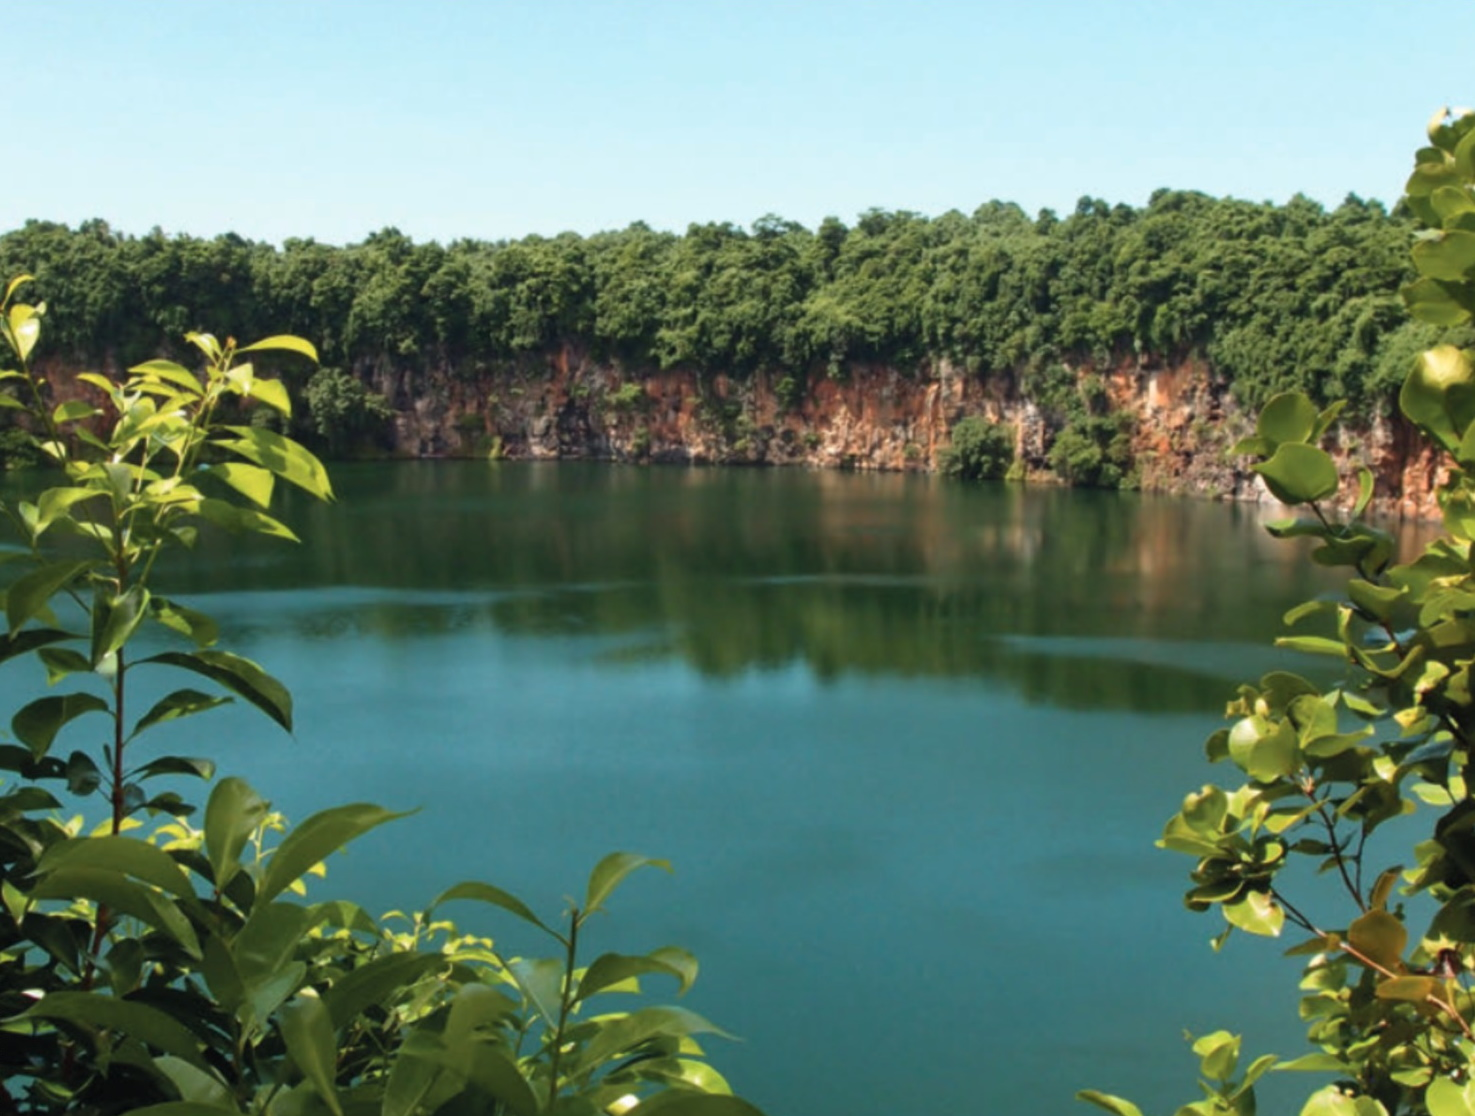
\includegraphics[width=0.8\linewidth]{lago_lalolalo}
	\caption{Lago Lalolalo}
\end{figure}

Il lago Lalolalo presenta una profondità di \(\SI{80}{\m}\) e sembra avere una stratificazione permanente: la sua zona eufotica (dove la luce è sufficiente perché sia possibile la fotosintesi) arriva fino a \(\SI{4}{\m}\), invece la zona anossica (in assenza di ossigeno)fino ai \(\SI{10}{\m}\).
Esso ospita 3 specie di pesci: Tilapia Oreochromis mossambicus, un guppy Poecilia reticulata (introdotto) e Anguilla oscura.
Va notato inoltre che gli immediati dintorni di Lanutavake e Lano presentano le ultime zone di esistenza delle foreste primarie dell'isola.

I laghi depressivi, ovvero quelli paludosi, sono due e si trovano sulla costa orientale dell'isola.
Essi rappresentano una preziosa riserva di acqua dolce.
I bordi di tali laghi  ospitano la popolazione della rana Litoria aurea, unica specie di anfibi presente sull'isola. 
Questa specie introdotta è originaria dell'Australia orientale e dell'Isola del Nord della Nuova Zelanda ed è l'unico vertebrato anfibio dell'isola di Uvea.

Alcuni laghi sono legati ad una falda acquifera sotterranea sottostante l'intera isola, che è alimentata dalle piogge e che si trova sovrapposta a una falda acquifera più profonda di acqua marina.
L'avifauna dell'isola di Uvea è relativamente povera e non comprende specie endemiche rigorose. 
Le rive dei laghi depressivi, in particolare Kikila, concentrano alcune specie, come la coda di paglia dalla coda bianca (Phaethon lepturus) e la gallina sultanina (Porphyrio porphyrio).
In alcuni laghi si trovano anche piccoli crostacei (Ostracodes) e Odonates come Ischnura aurora (Coenagrionidae).

\paragraph{RETTILI:}
I rettili sono rappresentati principalmente dagli scinchi e dai gechi.
Tra questi alcune specie endemiche delle Fiji e delle isole Wallis e Futuna sono classificati come EN (in via di estinzione) nella Lista Rossa IUCN (2014).
I resti delle fitte foreste rendono probabile però la presenza di altre specie endemiche non ancora scoperte.
Sull'isola sono presenti anche altre specie di rettili, come il piccolo serpente Indotyphlops braminus (ex Ramphotyphlops braminus).

\paragraph{INSETTI}
Sono stati identificati un totale di 211 artropodi e insetti su Wallis, Futuna e Alofi, di cui solo 6 sono considerati endemici: il ragno Schizocosa vulpecula, una cicala, Baeturia uvaeiensis endemica di Uvea, due coleotteri e altri due artropodi.
80 specie sono considerate autoctone e 125 sono specie introdotte.
Questo numero particolarmente basso mette in evidenza la necessità di ulteriori indagini.

\paragraph{UCCELLI}
Tutte e tre le isole hanno un numero inferiore di uccelli terrestri riproduttori e marini rispetto alle altre isole del Pacifico.
L'Aplonis tabuensis fortunae, o storno dalla Polinesia, è dei pochi esempi (se non l'unico) di sottospecie endemica specifica di Wallis, Alofi e futuna.

\paragraph{FAUNA MARITTIMA}
\subparagraph{CROSTACEI}
Wallis ha 31 specie di molluschi terrestri e quattro specie di acqua dolce.
Sull'isola le principali aree rimaste di biodiversità endemica delle lumache sono il Monte Loka, le macchie di foresta del monte Lulu Fakahega, il perimetro del Lago di Lano e del Lago di Lalolalo.
Inoltre ci sono circa 19 specie di cetrioli di mare.

\subparagraph{PESCI}
Nel 1999 e nel 2000, a Wallis, sono state registrate 648 specie di pesci di scogliera e laguna. Di queste specie, almeno 15 sono endemiche.
Le famiglie più presenti sono Gobiidac (74 specie), Labridae (61), Pomacentridae (57) e Apogonidae (49).
La maggior parte delle specie di grandi dimensioni e quelle che si trovano tipicamente nuotando sopra il substrato sono state registrate solo dal censimento visivo, come quasi tutte le specie delle famiglie Carangidae, Cac sionidae, Lethrinidae, Chaetodontidae, Scaridae, Scombridae e Tetraodonti das.

\subsubsection{Paesaggi culturali}
% \paragraph{SITI ARCHEOLOGICI} 
\subparagraph{Forte di Kolo Nui} \phantom{a}\\
Negli anni '90, i ricercatori del CNRS e del Nouméa Development Research Institute hanno effettuato scavi nel territorio di Wallis.

Uno dei principali siti archeologici di Wallis è il forte tongano di Kolo Nui a Talietumu nel distretto di Mu'a.
Questo è situato nella parte sud-occidentale dell'Oceano Pacifico, a nord-est rispetto a Halalo e a circa 9 km a sud-ovest dalla capitale Mata-Utu. 
Era un insediamento fortificato tongano con più ingressi circondato da mura difensive costruite in basalto.
Si ritiene che sia stato costruito intorno al 1450, durante l'espansione dell'Impero Tu'i Tonga, e che sia stata l'ultima resistenza dei tongani su Uvea, fino a quando non sono stati sconfitti.

\begin{figure}[ht]\centering
	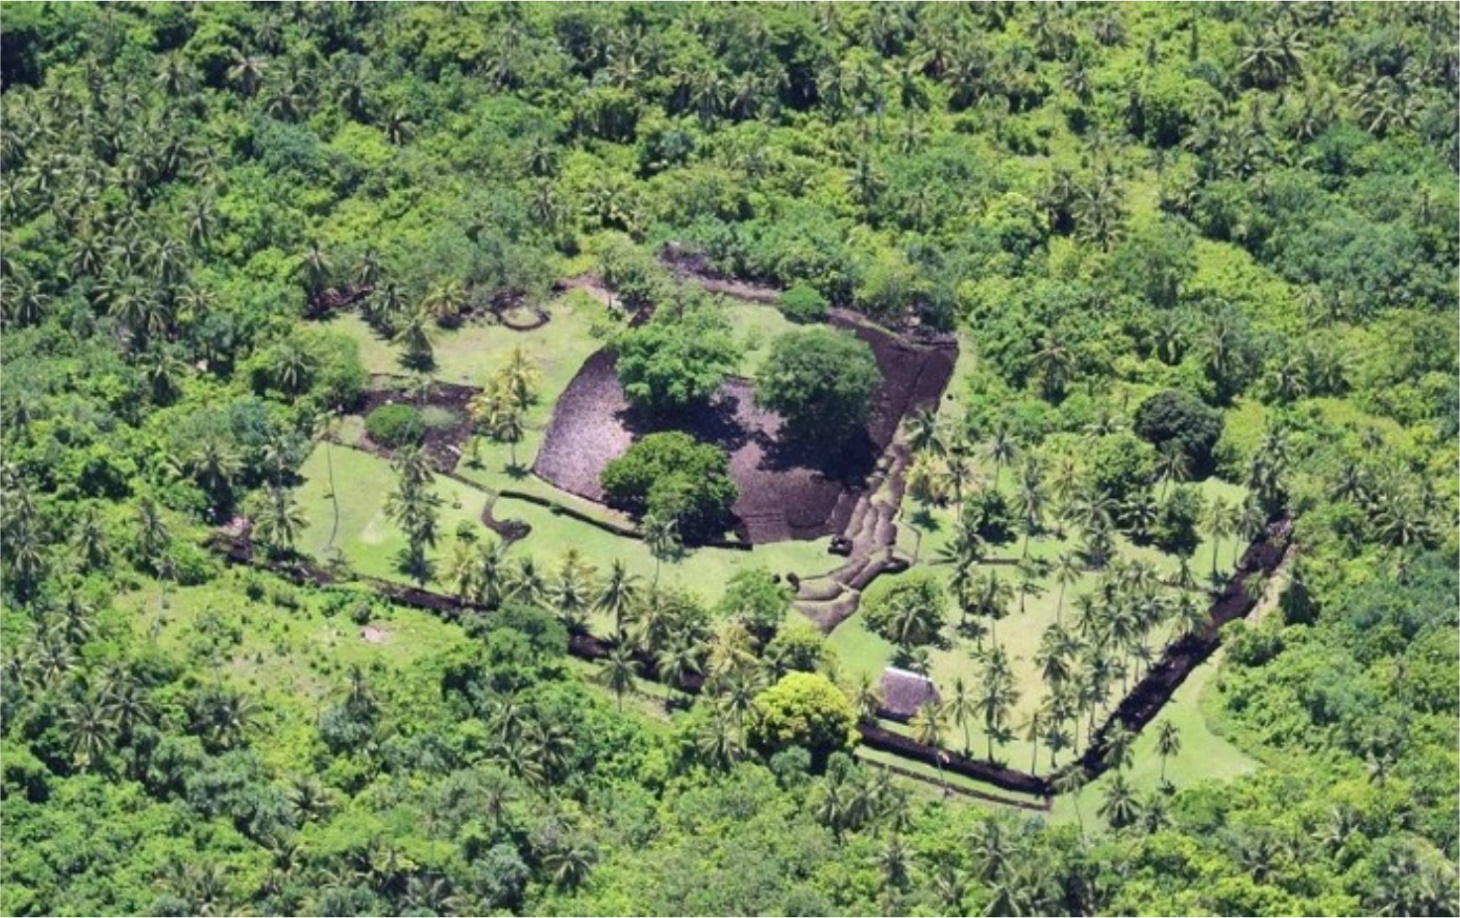
\includegraphics[width=0.8\linewidth]{kolo_nui}
	\caption{Forte di Kolo Nui}
\end{figure}

\subparagraph{La piattaforma Mālamatagata} \phantom{a} \\
La piattaforma Malamatagata si trova alle spalle della spiaggia dell'Utuleve, sulla costa occidentale.
Tale piattaforma è un monumento rettangolare, di circa \(\SI{30}{\m}\) per \(\SI{15}{\m}\), esteso da un basso collegamento in pietra (fatto probabilmente per permettere ai nobili di non muoversi allo stesso livello dei popolani).
Questo vicolo, deteriorato a causa delle coltivazioni, si unisce alla palude del To'ogatoto in cui sono presenti diverse strutture (tra cui un pozzo e recinti in pietra) destinate, secondo la tradizione orale, alla balneazione dei nobili.

\paragraph{SITI RELIGIOSI}
La costruzione di chiese sul territorio può considerarsi un arte. Le chiese, presenti in ogni distretto e in ogni villaggio, sono tutte diverse tra loro e per lo più realizzate con pietre vulcaniche molto colorate e scolpite a mano.
A Wallis i monumenti religiosi sono circa 26. 
La diocesi di Wallis e Futuna ha una cattedrale, situata a Mata Utu (Wallis), e una basilica dedicata a Pierre Chanel Poi.

\begin{figure}[ht]\centering
	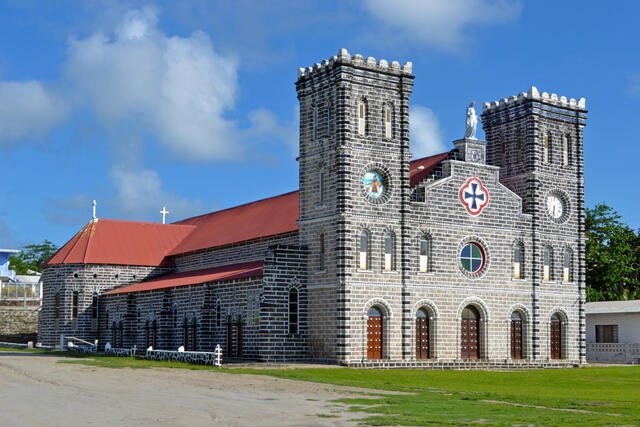
\includegraphics[width=0.8\linewidth]{mata_utu}
	\caption{Cattedrale di Mata Utu}
\end{figure}

\paragraph{ANALISI DELLA AREE ABITATE}
La popolazione conta 8084 abitanti di origine polinesiana, ed è divisa in tre distretti: Hihifo, Hahake e Sud Mua.
La parte occidentale è disabitata, le abitazioni si trovano sulla costa della costa orientale; parte della popolazione infatti vive ancora nelle "Fale Houses", ossia delle abitazioni ovali fatte interamente di paglia.

\paragraph{AREE PROTETTE}
Ad oggi non è stata istituita alcuna area protetta, tuttavia la comunità ha definito un quadro che ha permesso di preservare e valorizzare la biodiversità.
La comunità di Wallis e Futuna, infatti, ha istituito di recente una normativa in materia di tutela degli spazi naturali: il Codice dell'Ambiente è stato adottato dall'Assemblea territoriale il 26 luglio 2007.

Le disposizioni generali in materia di spazi e di aree naturali definiscono il termine "area protetta" come una "porzione di ambiente terrestre o marino, appositamente designata alla protezione e il mantenimento della diversità biologica, delle risorse naturali e culturali associate, e amministrato con mezzi efficaci, legali o altri" (Articolo E. 311-1).
In tale contesto, "la conservazione, la valorizzazione e la  gestione degli spazi naturali e paesaggistici del territorio hanno quindi lo scopo di proteggere tali territori da possibili minacce, la maggior parte delle quali sono la conseguenza di attività umane" (Articolo E. 312-1). 
Il Codice dell'Ambiente specifica che "lo stabilimento delle aree protette riguarda i siti e gli spazi che presentano un interesse per la conservazione della diversità biologica, in particolare consentendo la protezione delle specie e del loro habitat, più in generale per qualsiasi domanda ambientale, economica, sociale, culturale o estetica" (Articolo E. 321-1).

\subsubsection{Diritto fondiario}
Il diritto alla terra è consuetudinario, ossia non è regolato da leggi scritte ma da comportamenti ripetuti nel tempo con la convinzione di adempiere ad un obbligo giuridico. 
Nei villaggi sono presenti strisce di terra di proprietà di un insieme di individui strettamente imparentati tra di loro; altri terreni, situati più all'interno, hanno invece un legame stretto con alcuni gruppi di parentela, sono coltivabili e/o edificabili e il loro accesso è regolato dal gruppo stesso nel suo insieme che, di norma, decide per mezzo del "decano" del gruppo, di solito l'individuo più anziano, il quale va interpellato prima di prendere ogni decisione. 

\begin{figure}[ht]\centering
	\begin{tikzpicture}
		\pie[scale=0.8]{
			41.643/Foreste,
			15.5/Incolto,
			42.857/Arativo}
	\end{tikzpicture}
	\caption{Uso del suolo nell'isola di Wallis}
	\label{fig:wallis_land}
\end{figure}


Esistono poi ulteriori terreni che non sono assegnati a gruppi di parentela ma a uno chef coutumier, un capo consuetudinario.  
Non esiste una mappa precisa che definisce con precisione limiti e confini di questi terreni che la maggior parte delle volte non possono essere acquistati, ma vengono solitamente fatte delle convenzioni con concessioni molto lunghe, in alcuni casi fino a 99 anni. 

In questo contesto ha molta importanza anche il ruolo della Chiesa, la quale dispone di diversi terre con uno statuto differente.

\subsubsection{Consumi energetici}
Attraverso la legge statutaria del 1961, relativa ai poteri dell'assemblea territoriale, si è stabilito che lo Stato è l'unico competente in materia di energia.
L'ordinanza del 12 maggio 2016 estende e adegua alle isole Wallis e Futuna diverse disposizioni del Codice dell'energia.
Questa ordinanza ha tre conseguenze molto concrete per la popolazione e il territorio delle isole Wallis e Futuna:
\begin{itemize}
	\item nel 2020 le tariffe regolamentate per la vendita di energia elettrica al netto delle tasse sono state allineate a quelle della Francia continentale
	\item La transizione energetica a Wallis mira a raggiungere il \(\SI{50}{\percent}\) di energia rinnovabile entro il 2030 e l'autonomia energetica entro il 2050
\end{itemize}
L'attuazione dell'obbligo di acquisto di energia elettrica prodotta da fonti rinnovabili favorirà lo sviluppo di energie rinnovabili per il raggiungimento degli obiettivi prefissati. 

Gli idrocarburi consumati nel Territorio sono benzina, diesel e jet A1. 
Il diesel è il combustibile più utilizzato e rappresenta il \(\SI{70}{\percent}\) del consumo totale di idrocarburi dell'arcipelago. 
La società EEFW lo utilizza per la produzione di energia elettrica, che da sola rappresenta più del \(\SI{65}{\percent}\) del consumo a Wallis e Futuna.
Il consumo unitario o il consumo medio per cliente è di \(\SI{4.7}{\MWh}\) all'anno.
Il consumo totale energetico annuo di Wallis è di \(\SI{15.4}{\GWh}\) \cite{MagicFrenchDoc}.
Va notato che diversi grandi consumatori producono la propria elettricità.

\subsubsection{Produzione di energia}
Wallis e Futuna sono elettrificate e non sono interconnesse tra di loro, costituendo due sistemi elettrici e reti completamente separati.
Poiché la maggior parte della popolazione si trova a Wallis, anche la domanda di energia è più alta.

Fino al 2016, EEFW non è stato soggetto a revisione dei costi da parte della Commissione di regolamentazione dell'energia.
SWAFEPP è responsabile dello stoccaggio e della distribuzione di idrocarburi a Wallis e Futuna. 
Il carburante viene fornito da una petroliera delle Fiji.

I prezzi sono gli stessi sia a Wallis che Futuna, circa ogni tre mesi viene fissato il prezzo massimo tramite un decreto.
La struttura dei prezzi dei prodotti petroliferi è determinata tramite una deliberazione dell'Assemblea territoriale.
Il prezzo al dettaglio risulta dalla somma di tutti i costi intermedi: costo di importazione, tasse, costo dei servizi locali e margine degli addetti alle stazioni di servizio; per quanto riguarda il gas, la struttura si basa sullo stesso principio.

A Wallis il parco produttivo della centrale termoelettrica è composto da 7 generatori con una capacità installata totale di \(\SI{6.78}{\MW}\).
I due gruppi più importanti hanno un potere di \(\SI{1.25}{\MW}\). 
La potenza garantita in caso di mancanza di due motori è quindi di \(\SI{4.28}{\MW}\).
Sono in corso diverse azioni per migliorare la distribuzione dell'energia elettrica, tra cui l'interramento della rete MT e il parziale rinnovamento della rete di distribuzione con la sostituzione di 58 stazioni di trasformazione giunte a saturazione per un importo di quasi \(\SI{1200000}{\EUR}\) (150 MFCFP).

Per quanto riguarda le fonti rinnovabili a Wallis oggi si sfrutta solo l'energia fotovoltaica proveniente dal progetto TEP VERTES (sostenuto dall'Unione Europea), con una potenza installata di \(\SI{128}{\kWp}\); inoltre sono anche stati individuati due progetti di sviluppo di energie rinnovabili che utilizzano energie rinnovabili stabili:
\begin{itemize}
	\item Un progetto per una centrale elettrica da 500kW che sfrutta la biomassa situata a Malaé, il quale potrebbe essere sviluppato gradualmente, da \(\SI{100}{\kW}\) a \(\SI{150}{\kW}\) per testare e seguire la sua evoluzione e affidabilità.
	\item Un progetto per il recupero di rifiuti verdi, liquame e svuotamento di fosse settiche da cui si può ricavare biogas per fornire più di \(\SI{100}{\kW}\).
\end{itemize}

L'obiettivo attuale è quello di sviluppare \(\SI{3}{\MW}\) di fotovoltaico dando priorità a quello su tetto.
L'EEFW ha redatto un inventario degli edifici pubblici elencando le superfici dei tetti e il potenziale fotovoltaico per quanto riguarda l'orientamento, lo stato dei tetti e dei pendii.
Sono stati individuati più di trenta siti con una potenza dell'ordine di \(\SI{2}{\MW}\), di cui 9 siti con potenza superiore a \(\SI{100}{\kWp}\).
Numerosi edifici privati di natura commerciale hanno un grande potenziale per lo sviluppo del fotovoltaico su tetto.

\subsubsection{Disponibilità e produttività da tecnologie FER}
Da un'analisi preliminare condotta sulle tecnologie a nostra disposizione, si ottiene questa distribuzione del CF medio per tecnologia: 

\begin{table}[H]
	\caption{CF Medi annuali per Wallis}
	\centering
	\begin{tabular}{llc}
		\toprule
		Tecnologia   & CF \\
		\midrule
		Solare       & \(\SI{17.73}{\percent}\)         \\
		Eolico Offshore Palificato & \(\SI{30.14}{\percent}\)          \\
		WEC          & \(\SI{17.48}{\percent}\)         \\
		\bottomrule
	\end{tabular}
	\label{tab:wallis_cf}
\end{table}

Come si può notare da ciò, e dai dati di Global Wind Atlas, Wallis è un'isola con grande disponibilità di energia eolica.
Per quanto concerne invece il solare e il WEC, nonostante i due abbiano simili CF medi, il solare, dato il suo maggior sviluppo e minore LCOE, risulta essere un'altra ottima tecnologia da usare per garantire l'indipendenza dalle fonti non rinnovabili, risultando produttiva durante tutto l'anno.

\begin{figure}[H]\centering
	\begin{tikzpicture}
		\begin{axis}[ yshift = 1cm,
				% grid=both,
				axis lines = left,
				xlabel = {Mese},
				ylabel = {CF Medio [\%]},
				ybar interval,
				ymax=0.3,
				ymin=0,
				xmin=0,
				xmax=13,
				width=0.8\linewidth,
				% area style,
			]
			\addplot+[ybar interval, mark=no] table [
				x=month,
				y=cf,
				col sep=comma
			] {PlotsData/wallis_solar_monthly.csv};
		\end{axis}
	\end{tikzpicture}
	\caption{Produzione di solare media per ogni mese dell'anno nell'isola di Wallis}
	\label{fig:monthly_solar_wallis}
\end{figure}

\begin{figure}[ht]\centering
	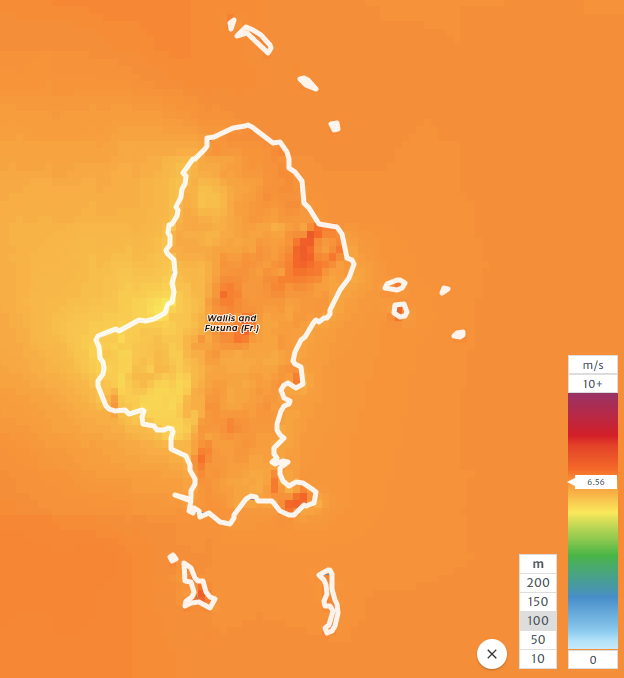
\includegraphics[width=0.8\linewidth]{wallis_wind}
	\caption{Mappa dei venti medi di Wallis, da Global Wind Atlas}
	\label{fig:wind_wallis}
\end{figure}

\subsubsection{Mercato energetico}
Il Codice energetico attribuisce all'isola di Wallis lo status di zona non interconnessa (ZNI) alla rete elettrica metropolitana continentale.
A Wallis, la società EEWF (Water and Electricity of Wallis and Futuna, filiale del Gruppo Engie) è responsabile dell'investimento, della gestione della produzione e della distribuzione di elettricità.
EEFW acquista tutta l'energia elettrica prodotta sul territorio insulare, gestisce continuamente l'equilibrio tra domanda e offerta di energia elettrica e ne assicura la trasmissione, distribuzione e fornitura a tutti i clienti. 
Come negli altri ZNI, i costi di produzione e di elettricità sono significativamente più alti di quelli osservati nella Francia continentale.

\subsection{Contesto socio-culturale}
\subsubsection{Storia coloniale, decoloniale, post-coloniale.}
I primi abitanti di Wallis furono austronesiani appartenenti alla civiltà di Lapita, che arrivarono a Wallis intorno al I millennio aC.
Tali abitanti formarono con gli arcipelaghi circostanti la "società ancestrale polinesiana".
Uvea fu poi integrata in una vasta rete di scambi (con varie isole della Polinesia) che si protrassero fino alla metà del 19° secolo con l'arrivo dei missionari europei.
Questi polinesiani ancestrali si impossessarono delle terre e cominciarono a sfruttarle, raccogliendo varie piante (taros, igname...) su fertili terre vulcaniche.
Tutti questi popoli parlavano la stessa lingua, il proto-polinesiano.

Dall'anno 1000 seguì un secondo periodo, chiamato "Atuvalu", che durò fino al 1400, e durante il quale gli Uvei passarono da un'economia di pesca e raccolta ad un'economia incentrata sull'agricoltura, in particolare sulla coltivazione del taro. 
Queste trasformazioni dello spazio e del sistema produttivo portarono a importanti ripercussioni sociali, tra cui la nascita del regno di Uvea, con un capo gerarchico.

Ai primi "chefferie" autonomi, nel sud e nel nord dell'isola, succedettero i primi "re" (in Wallisiano hau) di Uvea.
A tutto ciò poi seguì la conquista tongana di Wallis. 
Per stabilire il loro dominio, i tongani occuparono e costruirono molti forti come Kolonui, per questo motivo tale periodo viene chiamato ancora il "periodo dei forti".
L'occupazione si fermò poi intorno al 1500, con l'instaurazione di un sistema politico dinastico modellato sul modello tongano: un chiefdom di tipo piramidale, guidato da un hau.
È dal periodo dinastico, intorno al 1500, che iniziarono le genealogie dei successivi re di Wallis (Lavelua).
Solo la chefferie settentrionale (Hihifo) rimase indipendente e questa resistenza portò a numerosi conflitti, tra cui la guerra di Molihina, una guerra di indipendenza contro il dominio politico tongano.
I tongani imposero gradualmente la loro struttura sociale; la lingua wallisana si trasformò in profondità, integrando molti elementi del tongano.

L'influenza tongana ebbe conseguenze durature sulla storia locale, ma dopo circa un secolo dalla conquista tongana, Uvea ottenne gradualmente l'autonomia da Tonga, fino a quando uno dei Tu'i Tonga proclamò l'indipendenza dell'isola.
Il capitano britannico Samuel Wallis fu il primo europeo a sbarcare sull'isola nell'agosto del 1767. 
Fu per questo motivo che il suo equipaggio decise di nominare l'isola in suo onore.
A quel tempo Uvea contava \(\SI{4000}{}\) abitanti e rimase in gran parte isolata dai contatti tra polinesiani e occidentali, il che spiega anche il motivo per cui l'isola riuscì a mantenere la sua cultura e non subì una colonizzazione europea in senso stretto.

\begin{figure}[ht]\centering
	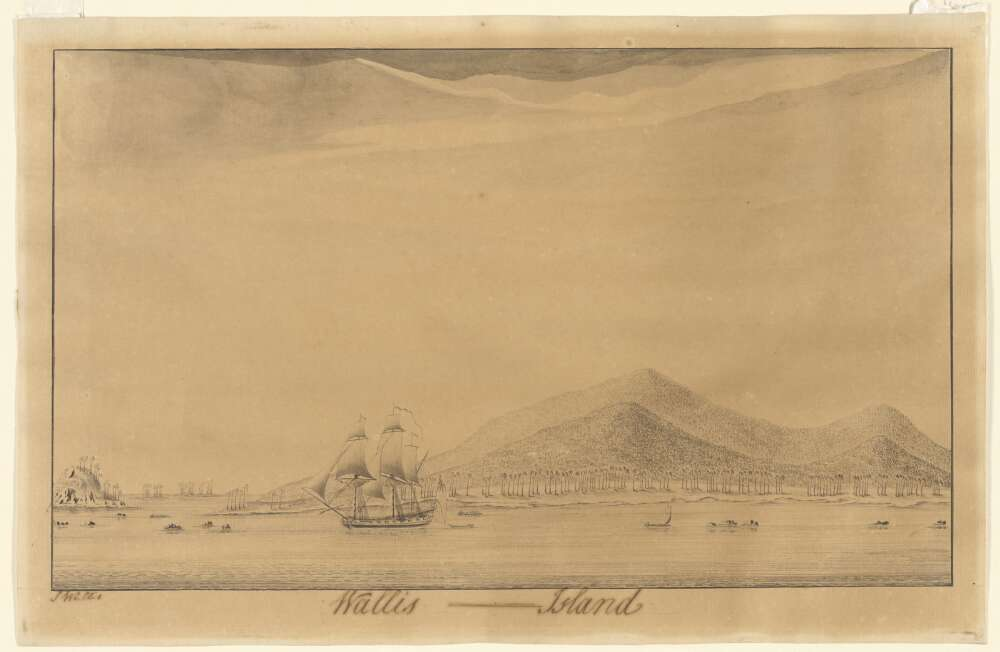
\includegraphics[width=0.8\linewidth]{wallis_drawing}
	\caption{Disegno di Wallis realizzato dal Capitano Samuel Wallis, 1767}
	\label{fig:wallis_drawing}
\end{figure}

Nel corso del diciannovesimo secolo a Wallis e Futuna iniziarono ad arrivare i marinai disertori dall'occidente.
I capi a sud di Wallis, dove si avvicinarono le barche, acquisirono abbastanza rapidamente un potere importante. Alcuni Wallisiani iniziarono a parlare anche inglese potendo così controllare il commercio estero, anche se ciò comunque destabilizzò i Lavelua.
Gli incontri tra marinai occidentali (per lo più inglesi o americani) e polinesiani non furono però privi di scontri, talvolta sfociarono in massacri; il più noto è quello del 1830, in cui un mercante inglese acquistò l'isolotto di Nukuatea dove si insediò con il suo equipaggio, e, da quel momento in poi, si considerarono proprietari dell'isola e cercarono di riservarne l'uso a se stessi.
Tuttavia, questa modalità di possesso esclusivo non poteva esistere nella società tradizionale wallisiana e iniziarono gli scontri.

La presenza europea non fu significativa al 1842, ma da lì in poi si rafforzarono i rapporti tra l'isola di Wallis e la Francia
Wallis però fu anche oggetto di desiderio tedesco e inglese e ciò rappresentò un pericolo per la Francia, soprattutto in termini religiosi: l'opera religiosa a cui si dedicarono i francesi sull'isola poteva infatti essere seriamente compromessa se una potenza prevalentemente protestante fosse venuta a legiferare.

Il trattato del 19 novembre 1886, o più esattamente del 5 aprile 1887, stabiliva l'effettivo protettorato della Francia su Wallis.
Infine, il decreto del 5 marzo 1888 unificò questi due protettorati che divennero un unico protettorato, "delle isole Wallis e Futuna".
Nel corso dei primi anni del '900 ci furono diversi tentativi di annessione di Wallis alla Francia, che però non andarono a buon fine.
La seconda guerra mondiale poi provocò molti sconvolgimenti a Wallis.

Tomasi Kulimoetoke è una figura che ha segnato la storia di Wallis e Futuna, poiché fu sotto il suo regno che le due isole passarono dallo status di protettorato a quello di Territorio d'Oltremare.
Nel 1959 fu organizzato un referendum sul cambio di stato, e il "sì" vinse a stragrande maggioranza (\(\SI{100}{\percent}\) a Wallis).
Fondamentale fu lo statuto del 1961, poiché mantenne e riconobbe l'organizzazione tradizionale dell'isola (capogruppo e monarchia), il diritto consuetudinario per i civili e l'educazione cattolica.
Venne istituita un'assemblea territoriale eletta a suffragio universale con una ventina di membri.
A Wallis e Futuna furono assegnati anche un deputato e un senatore.
Il territorio fu rappresentato anche da un consigliere economico e sociale.

Wallis e Futuna beneficiarono quindi di uno status su misura, adattato all'organizzazione sociale e politica delle due isole.
La moneta, un tempo riservata agli europei e ad alcune famiglie di funzionari locali, divenne più abbondante.
La società wallisiana adottò rapidamente il modello della società dei consumi, provocando il proliferare di grandi aree di vendita (ipermercati) e il crescente indebitamento delle famiglie con le banche.
Successivamente, dopo la revisione costituzionale del 2003, Wallis entrò a far parte della collettività d'oltremare di Wallis e Futuna.

\subsubsection{Storia culturale, sociale, politica.}
Nel 20° secolo la popolazione di Wallis è aumentata costantemente: a partire dal 1942, grazie all'installazione di una base americana a Wallis, iniziò un periodo di grande prosperità, che favorì la natalità e ridusse notevolmente la mortalità.
Di conseguenza, Wallis conobbe una "esuberanza demografica" che portò a un aumento della popolazione del \(\SI{45}{\percent}\).
Il picco demografico è stato raggiunto recentemente, nel 2003.

Durante il censimento del 2018, c'erano \(\SI{11.558}{}\) abitanti per l'insieme delle isole Wallis e Futuna, di cui il \(\SI{72.1}{\percent}\) appartenenti all'isola di Wallis.
La forte emigrazione, combinata con l'aumento dell'aspettativa di vita alla nascita, ha portato a un invecchiamento della popolazione.
L'età media è aumentata da \(\SI{28}{}\) anni a \(\SI{32.2}{}\) anni tra il 2008 e il 2013. 

Essendo un territorio francese, la lingua ufficiale dell'isola è il francese mentre il dialetto è il wallisiano, tutelato dall'Accademia delle Lingue Vallisiane; l'inglese è assai diffuso dato che è parlato in molte isole limitrofe.
La pesca e l'agricoltura sono le principali attività sin dall'antichità, l'economia, infatti, si basa sulla prevalenza del settore primario.
Quasi l'\(\SI{80}{\percent}\) della popolazione vive di agricoltura, pesca o artigianato.
La pubblica amministrazione è la fonte del \(\SI{75}{\percent}\) dei posti di lavoro.
Il settore privato, dal canto suo, è ancora debole nella creazione di ricchezza, solo l'attività commerciale contribuisce in modo significativo all'economia locale e  impiega oltre 300 persone.
L'importazione di merci, inoltre, rappresenta oltre il \(\SI{90}{\percent}\) del consumo.
Una delle bevande più diffuse è la Kava, ricavata dalla pianta omonima pestando le foglie e mescolandole con l'acqua fredda, ottenendo così un liquido grigiastro da consumare il prima possibile; solitamente viene consumata durante rituali e cerimonie. 

Famosi in tutto mondo sono i capi realizzati in tapa, un tessuto tipico del Pacifico creato a partire dalla corteccia del gelso da carta o dell'albero del pane, che viene tagliata finemente, imbevuta d'acqua e infine battuta per ottenere fogli molto sottili da cui si ricava il tessuto vero e proprio, il quale poi viene decorato con diverse tecniche.

\begin{figure}[ht]\centering
	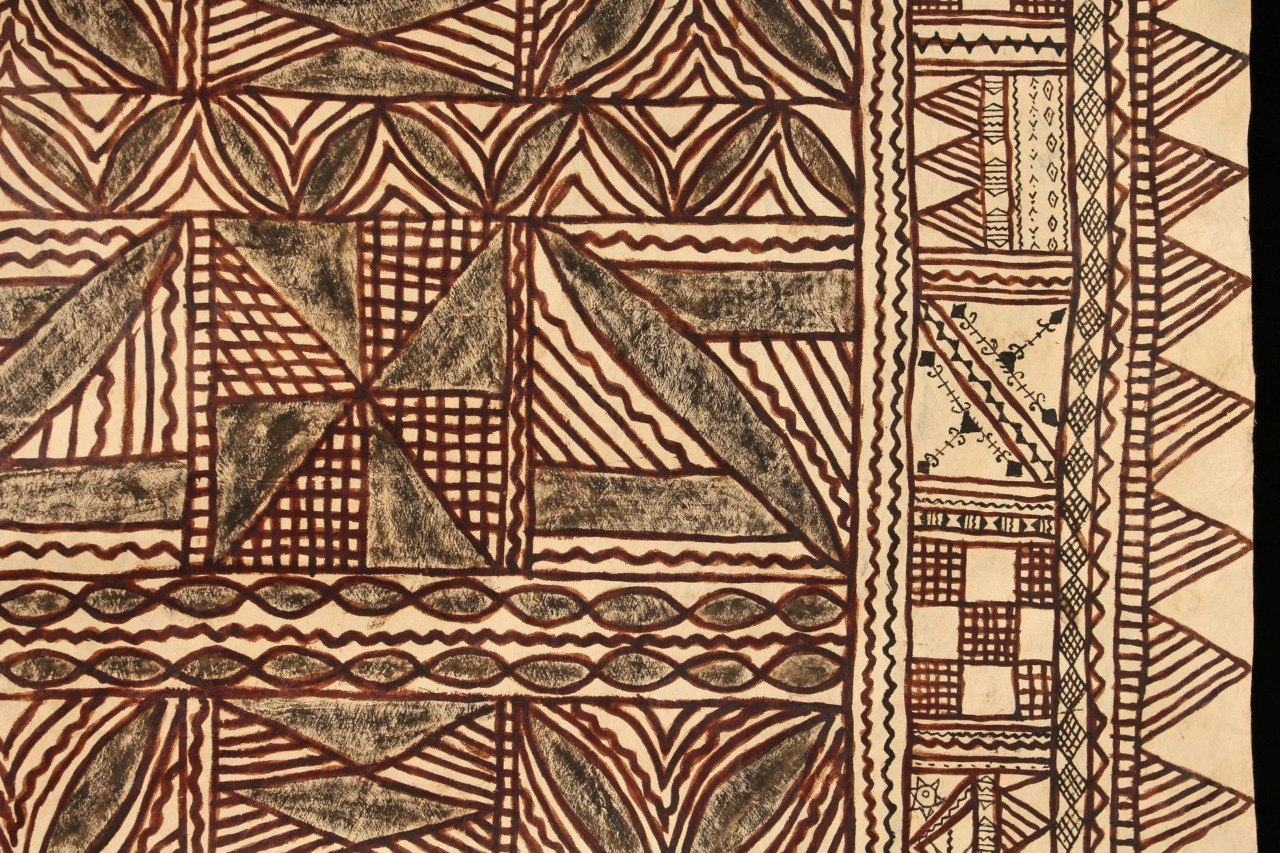
\includegraphics[width=0.8\linewidth]{tapa}
	\caption{Tessuto di Tapa}
	\label{fig:tapa}
\end{figure}

Sull'isola è presente un museo privato, l'Uvea Museum Association, collocato nella capitale Mata Utu, visitabile solo tramite appuntamento.
Al suo interno è possibile trovare oggetti che raccontano la storia di Wallis durante la seconda guerra mondiale, la maggior parte dei quali sono stati donati da veterani americani.
Per quanto riguarda l'istruzione, quella primaria è affidata alla Direzione dell'Educazione Cattolica (Pertanto è gratuita), mentre quella secondaria è gestita dal vicerettorato, mentre sono presenti soltanto un liceo di istruzione generale e un liceo agrario.
Gli studenti provengono anche dall'isola di Futuna.

La sanità è a carico dello Stato, e sul territorio sono presenti due ospedali e tre dispensari, anche se per le operazioni più specifiche spesso i pazienti vengono portati nelle strutture sanitarie della Nuova Caledonia.
Le risorse sanitarie sono comunque scarse e la popolazione soffre per il \(\SI{20}{\percent}\) di diabete, mentre l'\(\SI{80}{\percent}\) è sovrappeso, per questo motivo, nel marzo 2020, l'isola ha deciso di bloccare l'arrivo dei voli e l'assembramento di più di 100 persone, così facendo riuscì a non far circolare il virus sul territorio.

La religione di Wallis è il cattolicesimo, che da circa 200 anni ha sostituito le credenze tradizionali, e che svolge oggi un ruolo fondamentale all'interno della società.

\paragraph*{Contesto politico e ambientale attuale.}
Wallis e Futuna sono vulnerabili ai cambiamenti climatici.
L'estrazione di sabbia da parte dell'industria edile locale ha aumentato l'erosione della costa. 
Questo fenomeno, unito all'innalzamento delle acque, porta ad una riduzione della superficie abitabile, che richiederà lo spostamento delle popolazioni nell'entroterra.
I cicloni sono sempre più frequenti e alcuni si verificano anche fuori stagione, come il ciclone Ella nel 2017.
Il cambiamento climatico rischia inoltre di ridurre la produzione agricola, aumentando la dipendenza alimentare da prodotti importati.

In quanto territorio francese sul territorio dell'arcipelago vige la Costituzione francese del 1958, in particolare regalata dall'articolo 74 del titolo XIII.
Viene utilizzato il sistema legale francese ed il suffragio è universale per coloro che hanno superato l'età di 18 anni.
Il capo di stato è il Presidente Francese (Attualmente Emmanuel Macron), che viene eletto tramite un voto popolare presidente della Repubblica per un mandato di cinque anni.

Il Consiglio dei Territori è composto dai Re dei tre regni tradizionali (Uvea, Sigave, e Alo) e da tre membri nominati dall'Alto Amministratore su consiglio dell'Assemblea Territoriale.
Il potere legislativo è affidato all'Assemblea Territoriale unicamerale, i cui membri sono eletti con voto popolare ogni 5 anni.
Wallis e Futuna hanno diritto di eleggere un Senatore per il Senato francese e un deputato per l'Assemblea Nazionale francese.
I tre regni tradizionali amministrano la giustizia secondo leggi tradizionali (solo per illeciti non penali).
La corte d'appello si trova a Numea, in Nuova Caledonia. 
Il territorio, inoltre, partecipa al Segretariato delle comunità del Pacifico, un'organizzazione internazionale il cui scopo è quello di sviluppare le capacità tecniche, professionali, scientifiche e di gestione dei popoli delle isole del Pacifico, fornendo direttamente informazioni e consulenze circa il loro sviluppo e benessere.

L'economia di Wallis e Futuna è essenzialmente rurale. 
Fa parte di un'economia del dono e del controdono, in cui lo scambio di mercato è praticamente assente.
Grandi cerimonie consuetudinarie come il katoaga consentono la circolazione della ricchezza e una riaffermazione dell'ordine sociale.
Il valore dei beni che vengono ostentatamente scambiati dipende dalle relazioni sociali e dal loro valore d'uso. 
L'antropologa Sophie Chave-Dartoen osserva quindi che "termini come 'ricchezza' e 'valuta' non hanno equivalenti nella lingua valliana e la loro traduzione pone un problema".
Per l'antropologo Patrick Vinton Kirch, queste cerimonie di scambio di merci costringono gli abitanti a produrre più di quanto sarebbe sufficiente per la loro sussistenza per avere sempre delle eccedenze da offrire.
Questo quindi modella la produzione agricola (igname, taro, ecc.) e i suoi sottoprodotti (stuoie e tapa).

L'Unione europea (UE) ha svolto un ruolo attivo nel finanziamento degli sforzi di adattamento climatico di Wallis e Futuna. Nell'ambito del Fondo europeo di sviluppo, l'UE fornisce oltre 16 milioni di euro per sostenere lo sviluppo economico e sociale, nonché infrastrutture potenziate e capacità istituzionali per pianificare ed eseguire misure di adattamento ai cambiamenti climatici.
Attraverso INTEGRE, l'iniziativa dell'UE per la gestione ambientale del Pacifico, Wallis e Futuna hanno lanciato un sistema integrato di gestione delle zone costiere volto a limitare l'erosione costiera, porre fine alle pratiche di pesca distruttive e controllare la rimozione della sabbia dalla costa. È uno sforzo che i finanziatori sperano di replicare in altre nazioni vulnerabili al clima.
Altri piani INTEGRE mirano ad aumentare le capacità di gestione dei rifiuti delle isole costruendo discariche per aiutare a prevenire l'erosione, istituire fattorie biologiche pilota per implementare processi agricoli sostenibili e aumentare la consapevolezza razionalizzando la diffusione di materiale per la prevenzione dei disastri e la sensibilizzazione al clima.

Dal 1976, l'occupazione pubblica è aumentata notevolmente, passando da meno di 400 posti di lavoro a un  mercato di \(\SI{4000}{}\) lavoratori.
Se ogni anno più di 300 nuovi giovani lasciano il sistema educativo, non vengono creati più di 15 nuovi posti di lavoro. 
Inoltre, questa significativa disoccupazione è compensata da un massiccio esodo della popolazione, in particolare dei giovani che stanno tentando la fortuna in Nuova Caledonia, in Australia, o direttamente nella Francia metropolitana. 
Per visitare l'entroterra non ci sono mezzi pubblici, per questo motivo è necessario noleggiare un'auto, disponibili in entrambe le isole, anche se a Futuna non esistono agenzie ufficiali.
Non esiste il noleggio di bici o scooter.
Sono presenti un aeroporto e un porto.

\subsection{Modellazione energetica}

\subsubsection{Scenari: ipotesi}
Tramite la metodologia descritta in appendice, si ottengono i seguenti risultati per i valori delle potenze installate delle tecnologie prese in analisi e della capacità massima dello storage:
\begin{table}[H]
	\caption{Progetto proposto per Wallis}
	\centering
	\begin{tabular}{llc}
		\toprule
		Tecnologia   & Potenza/Capacità Installata \\
		\midrule
		Solare       & \(\SI{9.18}{\MW}\)         \\
		Eolico Offshore Palificato & \(\SI{2.00}{\MW}\) \\
		WEC          & \(\SI{0.00}{\MW}\)         \\
		Accumulatori & \(\SI{26.70}{\MWh}\)        \\
		Potenza Accumulatori & \(\SI{6.10}{\MW}\)   \\
		\bottomrule
	\end{tabular}
	\label{tab:wallis_project}
\end{table}

Si noti che, per quanto riguarda l'eolico, il valore di potenza installata è stato arrotondato all'intero più vicino, in quanto non si dispone di turbine con potenze intermedie.

Per l'isola di Wallis, dunque, l'energia solare è quella che risulta avere più successo, seguita dall'eolico e infine dall'energia da moto ondoso, che l'algoritmo esclude dalla soluzione ottimale.

I motivi di questa esclusione si ritengono essere principalmente legati al fatto che, rispetto al fotovoltaico e all'eolico (tecnologie ormai affermate con TRL pari a 9), il WEC, essendo stato sviluppato in tempi più recenti (TRL 6) presenta costi ancora troppo elevati per poter competere con le altre tecnologie.

Analizzati criticamente i dati ottenuti, inizia la fase di ricerca del sito di installazione per il fotovoltaico. 
Non avendo la possibilità di recarsi in prima persona sul campo, si conduce un'analisi preliminare sui luoghi da escludere a priori: tra questi figurano sicuramente i terreni a ridosso dei villaggi, concentrati lungo la costa orientale dell'isola, a sud-ovest i laghi vulcanici e le terre che le circondano, considerate Tapu dalla popolazione, e la zona del Forte Tongano, circa al centro dell'isola, tra i siti più belli del Pacifico nonostante la scarsa valorizzazione, tra l'altro contesa da più famiglie, la cui gestione è spesso motivo di tensioni nella popolazione.
Una volta esclusi questi terreni, al fine di avere il minor impatto ecologico possibile, vengono analizzate le zone già antropizzate dell'isola e tra queste la più appetibile risulta essere l'area vicino all'aeroporto indicata in figura \ref{fig:wallis_airport}.

\begin{figure}[ht]\centering
	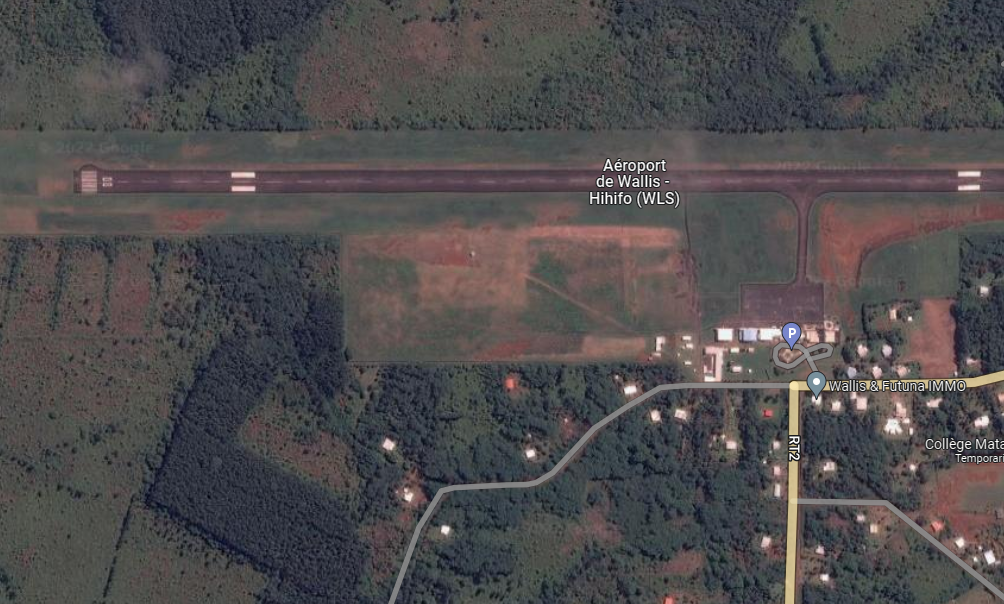
\includegraphics[width=0.8\linewidth]{wallis_airport}
	\caption{Aeroporto di Wallis, immagine di Google Maps}
	\label{fig:wallis_airport}
\end{figure}

Avendo accertato che quest'ultima risulta soddisfare i criteri di tipo ecologico-antropologico prefissati, si procede con la valutazione della potenza installabile. 
Per mezzo del software HELIOSCOPE che, selezionata manualmente la zona di installazione, fornisce la potenza di fotovoltaico installabile in quel sito, si ricava che la zona scelta ha una superficie più che sufficiente per ospitare i pannelli per la potenza richiesta, ragione per cui si ipotizza di sfruttare quest'area anche per l'installazione dello storage.
In caso, in seguito a un accesso al campo, la zona di terreno indicata non dovesse risultare sufficientemente estesa, verrà presa in considerazione l'iniziativa già presente sull'isola di installare fotovoltaico sui tetti di edifici abitativi e pubblici.

Per quanto concerne l'eolico, trattandosi di una tecnologia più invasiva dal punto di vista sia visivo che sonoro, un possibile sito può essere indicato solo in un secondo momento, dopo aver fatto un accesso diretto al campo, in modo da raccogliere più dati e avere un dialogo diretto con gli stakeholders del luogo. 
Viene, tuttavia, proposto un progetto di installazione, al momento testato a Taiwan dalla multinazionale danese Orsted, che, in un non così lontano futuro, potrebbe rivelarsi essere la soluzione ideale per Wallis. \cite{ORS:Coral}

\begin{figure}[ht]\centering
	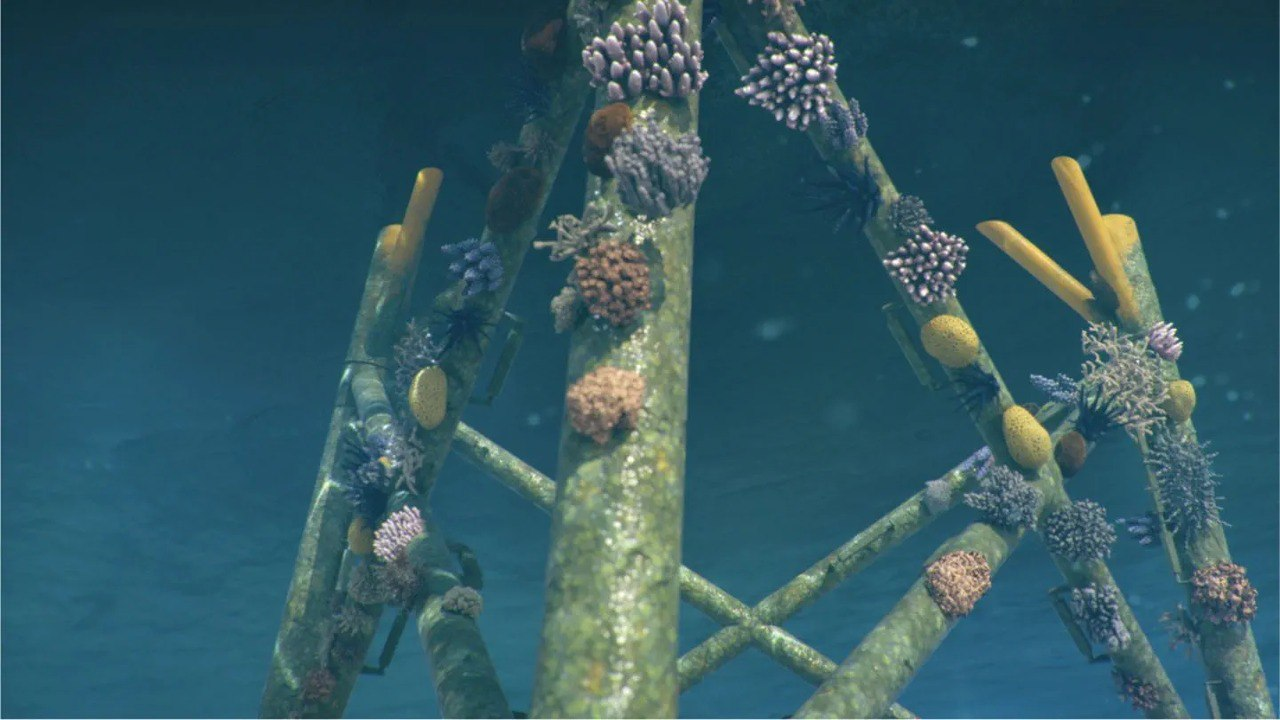
\includegraphics[width=0.8\linewidth]{turbina_coralli}
	\caption{Una turbina costruita sui coralli}
	\label{fig:coralli}
\end{figure}

L'isola è circondata dalla barriera corallina, dimora di una gamma vastissima di specie marine diverse, tra gli ecosistemi più ricchi in termini di biodiversità e non solo.
Il cambiamento climatico e l'innalzamento della temperatura, però, provocano sempre più frequentemente lo sbiancamento dei coralli, e ciò minaccia la sopravvivenza dell'intero ecosistema. 
A farne le spese non sono "solo" le centinaia di migliaia di specie marine il cui habitat naturale è la barriera corallina, ma anche milioni di persone il cui sostentamento dipende da queste specie, senza dimenticare che la presenza della barriera corallina protegge la costa da inondazioni e tempeste. 
Dalla necessità da un lato di produrre energia in modo green e, dall'altro, di salvaguardare queste specie e il loro ecosistema, nasce l'idea di popolare di coralli le basi che permettono l'installazione delle turbine eoliche in mare.

I coralli si trovano spontaneamente in acque superficiali, la cui temperatura molto elevata può causare il loro sbiancamento. 
Ma nelle acque più profonde, dove sarebbero installate le turbine, la temperatura si mantiene più bassa e stabile, grazie alla continua circolazione di acqua calda proveniente dalla superficie e di acqua fredda dal fondale.

Le fondamenta delle turbine offshore forniscono dunque un ambiente unico dove i coralli possono crescere, abbastanza vicini alla superficie in modo da ricevere sufficiente luce solare, ma senza essere esposti alle alte temperature. 
Tutto ciò non solo limiterebbe i rischi di sbiancamento dei coralli, ma li aiuterebbe anche a proliferare e, una volta maturi, a rilasciare le loro uova che, trasportate dalle correnti oceaniche, potrebbero depositarsi naturalmente su altri fondali. 
Si tratta inoltre di un approccio non invasivo, in quanto, per il popolamento, sono collezionate le uova di coralli che si depositano a riva e che non sopravviverebbero altrimenti, lasciando intatti gli ecosistemi corallini già esistenti.

Esistono ancora delle incertezze sul successo del progetto, quali l'ancoramento alle basi delle turbine delle larve dei coralli nonostante le forti correnti o il loro prosperare sebbene la collocazione sia meno luminosa rispetto a quella usuale, ma i benefici che questa soluzione porterebbe superano di gran lunga i possibili aspetti negativi.

Un'ultima riflessione è dedicata al WEC, per il quale, pur essendo sfavorito dall'algoritmo, è stata comunque presa in considerazione l'ipotesi di installazione. 
A causa della presenza della barriera corallina che riduce mediamente del \(\SI{97}{\percent}\) la potenza dell'onda oceanica e dell'\(\SI{84}{\percent}\) la sua altezza, in caso l'installazione avvenisse nella laguna, il dispositivo risulterebbe inutile. 
D'altro canto, invece, collocare il dispositivo al di là della barriera corallina risulta essere una scelta piuttosto rischiosa in quanto, in caso di cicloni o di altri eventi di natura estrema, non così rari nel Pacifico, un eventuale guasto degli ormeggi si potrebbe tradurre in un serio danno alla barriera.

Implementando la soluzione proposta, si otterrebbe un utilizzo delle energie rinnovabili del \(\SI{95.05}{\percent}\), con un LCOE stimato del progetto a \(\SI {0.079}{\EUR\per\kWh}\). L'energia consumata segue quindi una distribuzione come quella in figura \ref{fig:monthly_consumption_wallis}. \\
\begin{figure*}[ht]\centering
	\begin{tikzpicture}
		\begin{axis}[ 
				% yshift = 1cm,
				% axis lines = left,
				yshift = -1cm,
				xlabel = {Mese},
				ylabel = {Consumo [GWh]},
				ybar stacked,
				% ybar legend,
				% ymax=0.3,
				% ymin=0,
				% xmin=0,
				% xmax=13,
				% xmin=1,
				% xmax=12,
				date coordinates in=x,
				xtick=data,
				xticklabel={\pgfcalendar{tickcal}{\tick}{\tick}{\pgfcalendarshorthand{m}{.}}},
				width=0.8\linewidth,
				legend style={at={(0.5,-0.13)},
                    anchor=north,legend columns=-1},
				% area style,
			]

			\addplot+[ybar, mark=no, black, fill=RedOrange] table [
				x=month,
				y=solar,
				col sep=comma,
				y expr=\thisrow{solar}*1e-9,	
			] {PlotsData/wallis_consumption.csv};

			\addplot+[ybar, mark=no, black, fill=SeaGreen] table [
				x=month,
				y=wind,
				col sep=comma,
				y expr=\thisrow{wind}*1e-9,
			] {PlotsData/wallis_consumption.csv};

			% \addplot+[ybar, mark=no, black, fill=NavyBlue] table [
			% 	x=month,
			% 	y=wec,
			% 	col sep=comma,
			% 	y expr=\thisrow{wec}*1e-9,
			% ] {PlotsData/lipari_consumption.csv};

			\addplot+[ybar, mark=no, black, fill=yellow] table [
				x=month,
				y=accumulator,
				col sep=comma,
				y expr=\thisrow{accumulator}*1e-9,
			] {PlotsData/wallis_consumption.csv};

			\addplot+[ybar, mark=no, black, fill=black] table [
				x=month,
				y=diesel,
				col sep=comma,
				y expr=\thisrow{diesel}*1e-9,
			] {PlotsData/wallis_consumption.csv};

			\legend{Solare, Eolico, Accumulatori, Diesel}
		\end{axis}
	\end{tikzpicture}
	\caption{Consumo mensile per tecnologia nell'isola di Wallis}
	\label{fig:monthly_consumption_wallis}
\end{figure*}

\subsection{Strategia di accesso al campo e posizionamento}
Come anticipato nel punto precedente, la scelta dell'area per l'installazione di un tale impianto risulta particolarmente complicata e non può essere fatta interamente a priori, in quanto oltre all'aspetto prettamente burocratico legato alla sicurezza e alla tutela dell'ambiente, è necessario anche un confronto diretto con la popolazione e le istituzioni locali. 
Solo un accesso diretto al campo può infatti validare le ipotesi di installazione avanzate nella fase di modellazione. 

\subsubsection{Portatori di interesse (potere decisionale, influenza, obiettivi)}
Tra gli stakeholders vi è innanzitutto il Governo Francese, attraverso il suo rappresentante più importante, il prefetto, che è allo stesso tempo capo del territorio, coprendo una "doppia" carica politica locale e amministrativa davanti allo Stato francese; vi è inoltre un'Assemblea del territorio, ossia un parlamento locale di membri eletti. 
È poi presente un sistema complesso di capi locali rappresentato da un re, il "Lavelua", sovrano dell'isola e delle sue terre, insieme allo Stato francese e a un Consiglio di capi.

Un altro interlocutore fondamentale è il capo del "distretto" più strettamente interessato al luogo di interesse. 
Tra i portatori di interesse si ha anche la Chiesa, rappresentata dalla figura del Vescovo, la cui autorizzazione è necessaria per ogni progetto sull'isola.
Esistono anche assemblee di cittadini a cui si dovrà presentare il progetto, veri e propri sistemi politici in cui si discute molto, dal momento che i singoli individui vogliono essere informati e partecipi delle decisioni, il che allunga i tempi operativi, ma che rende l'intero progetto democraticamente produttivo.

Un ultimo importante stakeholder è la società EEWF, che detiene il monopolio della produzione e distribuzione dell'energia elettrica sull'isola.

I piani per l'evoluzione dell'energia rinnovabile devono allinearsi agli obiettivi nazionali e internazionali ma sempre tenendo presente il rispetto delle giurisdizioni del territorio.
L'obiettivo è quello di favorire uno sviluppo energetico sostenibile, preservando i valori ecologici e antropologici dell'isola. 
In un contesto di globalizzazione, l'isola deve riuscire a integrarsi senza però perdere la propria unicità in termini di biodiversità, storia e cultura. 
Un progetto, per potersi dire di successo, deve essere condiviso sia dalla popolazione locale che dalle istituzioni, rimanendo, in ogni sua fase, sostenibile dal punto di vista ambientale. 


\subsubsection{Legittimità e riconoscimento (pratiche, comportamenti e protocolli)}
Al fine della presentazione del progetto si ritiene necessario un doppio approccio "dall'alto", interpellando lo Stato francese, il re e le altre figure a capo dell'isola e delle sue terre  precedentemente indicate, e "dal basso" coinvolgendo la popolazione.
Per quanto concerne lo Stato, ci si deve attenere alle procedure amministrative, che solitamente sono quelle adottate anche in Francia, e di conseguenza è necessario presentare il progetto fornendo indicatori, vantaggi, svantaggi, e adottando quindi un approccio prettamente tecnico; per quanto riguarda invece il coinvolgimento della popolazione, la situazione è più complessa in quanto non esistono leggi scritte o protocolli precisi da seguire. 
È consigliato procurarsi innanzitutto un interlocutore, che solitamente è lo chef coutumier che ha il controllo dell'area interessata, che permetta di presentare il progetto sia ai cittadini che al Re. 
Senza l'approvazione di quest'ultimo e della figura del Vescovo non è possibile procedere, anche se non esistono leggi ufficiali a riguardo. 
Un aspetto fondamentale è la presentazione del progetto all'Assemblea cittadina, che può approvare solo con l'unanimità dei membri, infatti sull'isola, nell'ambito delle decisioni, al posto del concetto tipicamente europeo di maggioranza vale quello di consenso.


\subsection{Conclusioni}
\subsubsection{Limiti e opportunità}
Wallis presenta caratteristiche paesaggistiche uniche nel suo genere: la sua conformazione lagunare, che permette la formazione di una ricca barriera corallina che costeggia tutta l'isola, la presenza di diversi laghi craterici di origine vulcanica e la presenza di svariati siti archeologici e religiosi sono tutti aspetti che vanno presi in considerazione per affrontare un caso studio complesso come questo. 

La presenza della barriera corallina pone diverse sfide riguardo la disposizione delle tecnologie proposte, alla quale bisogna prestare particolare attenzione in quanto, tra i vari aspetti da valutare, bisogna mettere al primo posto la necessità di preservare ogni habitat naturale ed ecosistema natio. Inoltre i diversi siti archeologici, come il forte Tongano e le aree religiose, rappresentano siti inaccessibili alle ricerche scientifiche; a queste aree vanno aggiunti tutti i luoghi del "non detto", ovvero quelli in cui per la cultura e le tradizioni wallisiane non è possibile effettuare ricerche di alcun tipo. 

Oltre alle limitazioni di tipo ambientale e culturale vanno anche considerate tutte le disposizioni sociali e politiche: al fine della realizzazione del progetto è necessario instaurare un rapporto diretto da un lato con il principale stakeholder, ovvero il governo francese, e dall'altro con il re e le altre figure a capo dell'isola. 

E' necessario presentare all'interno del progetto tutti i possibili vantaggi e svantaggi. La parte più difficoltosa risulta l'approccio con la popolazione che non risulta regolamentato da alcuna legge o normativa. Tramite l'assemblea cittadina viene discussa e valutata la realizzabilità del progetto secondo gli interessi e il benessere dell'isola. È compito di coloro che avranno la possibilità di accedere al campo di rispettare tutti i protocolli e gli standard imposti affinché il rapporto ricercatore-popolazione sia di rispetto e proficuo per entrambe le parti.


\subsubsection{Analisi delle opzioni}

Dopo aver effettuato uno studio sinergico sulle attuali condizioni dell'isola sono state effettuate diverse considerazioni sia sull'approccio al campo che sui metodi di installazione delle tecnologie scelte. Ai fini della preservazione della barriera corallina è stata proposta una scelta del tutto innovativa già sperimentata in un altro contesto: l'impiego delle fondamenta delle turbine come habitat perfetto alla proliferazione dei coralli; se da un lato l'obiettivo è quello di ottimizzare le soluzioni energetiche dall'altro vi è l'ambizione di salvaguardare il paesaggio e l'ecosistema creando un equilibrio perfetto tra natura e tecnologia. 

Il fotovoltaico, secondo le analisi, risulta una tecnologia molto efficiente in termini sia di prestazioni che di costo, ciò è dovuto al fatto che possiede grande affidabilità nella produzione energetica, così come un LCOE molto basso, il che rende la tecnologia molto competitiva in termini economici. 
Dopo un'attenta analisi dei siti disponibili la scelta è ricaduta nelle zone limitrofe all'aeroporto: una zona perfetta perché a basso impatto visivo ed ecologico. 

Il WEC invece ha riscontrato poco successo in quanto il posizionamento dello stesso all'interno della laguna risulterebbe inefficace a causa dell'eccessivo smorzamento dell'onda marina causato proprio dalla presenza della barriera corallina, mentre il posizionamento al di fuori di quest'ultima risulterebbe poco agevole e rischioso in quanto potenzialmente dannoso alla barriera stessa; tutto ciò, in aggiunta al fatto che il WEC è una tecnologia in fase di sviluppo renderebbe un investimento in essa per Wallis alquanto rischioso.


Dalle considerazioni fatte si ottiene un impiego di energia rinnovabile pari al \(\SI{95.05}{\percent}\).


% ==================
% LIPARI
% ==================

\section{Isola di Lipari}
\subsection{Scopo}
Lo scopo di questa relazione è quello di analizzare dal punto di vista ecologico, antropologico ed energetico l'isola di Lipari, per poter formulare un'ipotesi di progetto di energie rinnovabili specifica sulla base del territorio, delle risorse e della popolazione che abita il luogo di interesse.

\subsubsection{Contesto territoriale}
L'isola di Lipari, anticamente definita Meligunis dai colonizzatori greci, è la più grande delle isole costituenti l'arcipelago delle Eolie. 
Presenta una superficie di \(\SI{37.6}{\km\squared}\) con circa 12000 abitanti residenti con  una densità media abitativa di \(\SI{136.7}{}\) \(\frac{\text{abitanti}}{km^2}\).  
Dai dati raccolti a partire dall'anno 2001 fino al 2020, è possibile notare come il numero di residenti nell'isola sia sommariamente sempre aumentato, per poi subire una leggera diminuzione (registrata nel periodo del Covid). 
Il principale nucleo abitativo dell'isola di Lipari si sviluppa lungo Marina Corta, Marina Lunga e la fortificazione del Castello; altri piccoli centri sono situati nelle contrade di Canneto, Pianoconte, Acquacalda e Quattropani, tutti collegati tra loro da un'efficiente rete stradale.

\begin{figure}[ht]\centering
	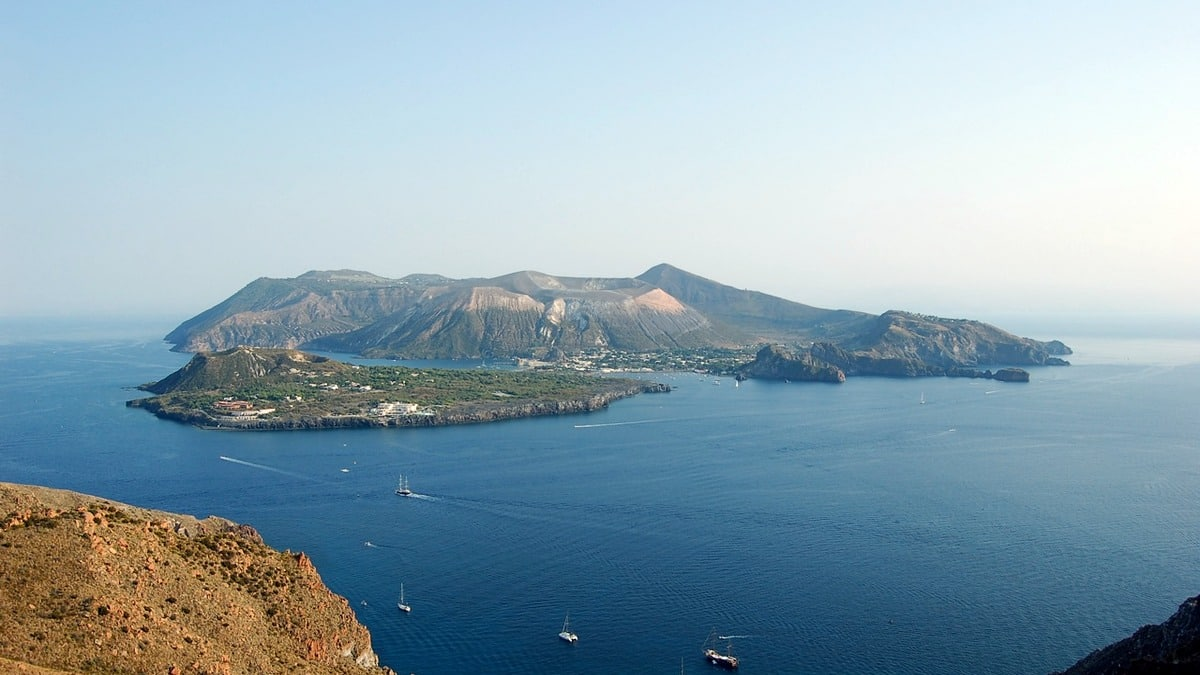
\includegraphics[width=0.8\linewidth]{lipari}
	\caption{Isola di Lipari}
	\label{fig:lipari}
\end{figure}

Un altro dato di fondamentale importanza riguarda l'analisi dei flussi migratori della popolazione. 
Dai grafici è possibile evidenziare la costante positività del saldo migratorio totale (il quale comprende sia i contributi dovuti alla migrazione da e per l'estero sia la migrazione da e per altre regioni) e del saldo migratorio con l'estero. 
Un po' più oscillante è invece l'analisi degli spostamenti tra Lipari e le altre regioni, che presenta picchi di massimi negli anni 2012 e 2013, riconducibili all'aumento copioso del turismo nazionale (\(\SI{+10}{\percent}\)) ed internazionale (\(\SI{+20}{\percent}\)). 
Questi numeri indicano che il turismo sia una delle attività di sostentamento più importanti dell'isola. 
Fino alla prima metà degli anni '50, a Lipari e in tutte le Eolie, l'economia era basata sull'agricoltura, sulla pesca ed estrazione della pietra pomice. 
Poi, a partire dal decennio successivo, la scelta di Lipari come scenografia per due film importanti quali "Stromboli, terra di Dio" del regista Roberto Rossellini, e "Vulcano" di William Dieterle, hanno suscitato un copioso interesse, facendo diventare l'isola un'ambita meta turistica.

\subsubsection{Biogeografia}
L'isola di Lipari è il risultato di una serie di eruzioni vulcaniche che si sono succedute nel corso dei millenni. Essa presenta coste alte e frastagliate, con numerosi scogli, grotte e faraglioni; la sua superficie ha forme molto irregolari, alcune montagne si separano solo in sommità, mentre altre appaiono totalmente indipendenti. I rilievi principali dell'isola sono Monte S. Angelo, Monte Chirica, Monte Pilato e Monte Mazzacaruso.

La flora vascolare conta 900 specie e non è difficile incontrare specie esotiche come eucalyptus, acacia e alnus. La popolazione floristica è composta in prevalenza da piante erbacee che costituiscono circa l'\(\SI{80}{\percent}\) del totale, mentre il restante \(\SI{20}{\percent}\) è composto da piante legnose. Dal punto di vista biogeografico ed ecologico, risultano essere di rilevante interesse le specie endemiche come la podarcis raffonei e l'elyomis quercinus liparensis. Nella zona di Pirrera si possono ammirare boschi autoctoni, i quali hanno contribuito a mantenere l'ecosistema integro nel suo aspetto naturale, essendo particolarmente difficile l'accesso per l'uomo a queste aree. Questi boschi sono composti principalmente da leccio, erica, caprifoglio. Negli anni, l'impoverimento del patrimonio boschivo ha portato la sostituzione delle piante arboree con la macchia Mediterranea, costituita dalla ginestra odorosa, da cisti e dall' endemica ginestra.

Una delle coltivazioni che si è contraddistinta nel corso dei secoli e che, ad oggi, rappresenta una grossa realtà produttiva, è quella del cappero (quest'ultimo viene esportato in apposite anfore sin dai tempi dei romani). Oltre ad essere uno dei perni della cucina locale, è una grossa fonte di reddito insieme alla malvasia.
Dal punto di vista faunistico, maggiore interesse viene attribuito alle specie endemiche, esclusivamente circoscritte al territorio eoliano. Ad oggi, il numero di esse si è ridotto notevolmente, e infatti le specie focali podarcis raffonei e le sue sottospecie di gliride, sono ancora individuabili in pochissimi tratti boschivi di Lipari. È presente un numero elevato di specie di invertebrati. Si trovano allo stato endemico cinque specie di coleotteri, una di lepidottero, una di omotteri, due di ragni disderidi, tre di collemboli e cinque di molluschi polmonati.

Nei periodi primaverili ed autunnali, si assiste al transito di uccelli migratori come oche selvatiche, quaglie, fenicotteri, pellicani, la Berta Maggiore, il Falco Mediterraneo, il Corvo Imperiale.

Una posizione di rilievo è assunta dalla lucertola delle Eolie, presente ormai in numeri molto ridotti, solo in poche aree a causa dell'introduzione della lucertola campestre (podarcis sicula) da parte dell'uomo.

Per quanto concerne la biogeografia marina, l'intensa attività vulcanica che contraddistingue l'arcipelago, composto da ben 12 vulcani collegati, ha modellato i fondali creando un ambiente caratterizzato da scogliere, vulcani sommersi e grotte. I fondali marini offrono pareti di ossidiana, distese di posidonia e colorazioni che variano dal bianco della pomice al nero della sabbia vulcanica.

L'elevata biodiversità della vegetazione marina e la presenza di alghe pelagiche costituiscono un ambiente ricco di insediamenti e di specie bentoniche e planctoniche, creando un ambiente perfetto di nidificazione per numerose specie ittiche quali: Aragosta, Astice, Calamaro, Cavalluccio marino, Cefalo, Cernia, Dentice, Gambero, Pesce spada, Polpo. Proprio grazie a questi, i cetacei trovano un ambiente ideale per la loro sopravvivenza. Le specie più comuni sono: il Capodoglio, il Delfino, la balenottera.


\subsubsection{Paesaggi culturali}
Per la sua posizione e per la sua estensione, Lipari è stata la prima delle isole Eolie ad essere abitata, dal \(\SI{5000}{}\) a.C., durante il neolitico medio e vide il susseguirsi di varie civiltà. E' l'isola più popolosa dell'arcipelago, e i suoi abitanti vivono in diversi centri abitati: Lipari centro, Pianoconte, Canneto, Quattropani, Acquacalda, Porticello.

L'abitato si estende ai piedi dell'imponente rocca del Castello, l'antica acropoli della città greca e romana, che si erge su alta roccia di lava, con bastioni a strapiombo sul mare. La fortezza naturale della rocca del Castello domina i due approdi dell'isola, le insenature naturali di Marina Lunga e Marina Corta, e conserva le testimonianze del passato, essendo stata abitata quasi ininterrottamente da \(\SI{6000}{}\) anni.

\begin{figure}[ht]\centering
	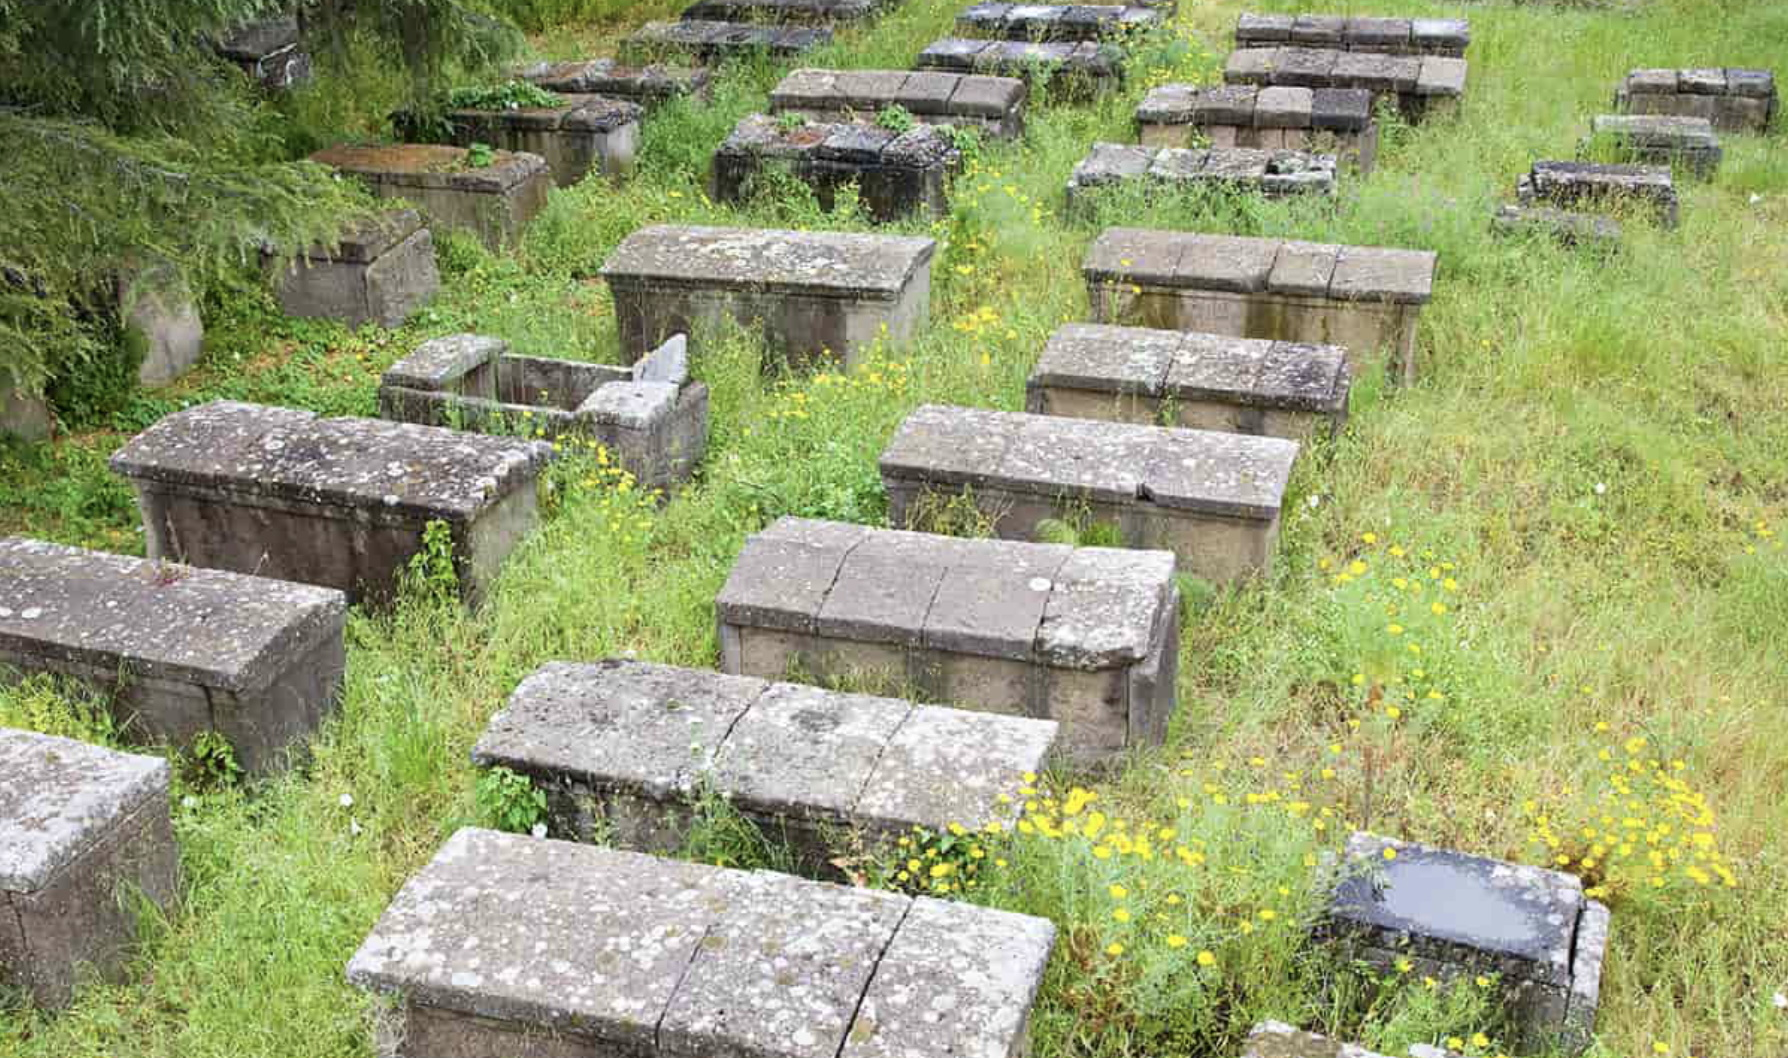
\includegraphics[width=0.8\linewidth]{necropoli}
	\caption{Necropoli di Lipari}
	\label{fig:necropoli}
\end{figure}

L'acropoli di Lipari costituisce ancora oggi il punto focale del centro storico; all' interno sono conservate la statua argentea di S. Bartolomeo ed una tavola del seicento raffigurante la Madonna del Rosario. Ancora più in fondo appare la chiesa della Madonna delle Grazie, chiusa al culto, che raccoglie diversi affreschi; il palazzo vescovile, del 1753, che è posto sul lato destro della cattedrale, è adibito a padiglione del museo.

La necropoli greca di Lipari che si estende nella pianura di Diana sottostante la rocca del Castello, è una delle più ricche della Sicilia: trent'anni di scavi hanno recuperato i corredi di oltre 1750 tombe, ora esposti al Museo Archeologico Regionale Eoliano. Quest'ultimo ha sede nel Castello e, creato nel 1954 da Luigi Bernabò Brea e Madeleine Cavalier, espone i reperti degli scavi condotti dal 1950 ad oggi a Lipari e nelle isole di Panarea, Salina, Filicudi e Stromboli. La sezione del Museo Eoliano, relativa alla preistoria dell'isola di Lipari, occupa l'antico palazzo vescovile adiacente alla Cattedrale.

La basilica concattedrale di San Bartolomeo è il principale luogo di culto di Lipari; sorge nel cuore della Cittadella ed è la più grande e antica delle chiese di Lipari. Alla prima edificazione pagana, risalente all'età ellenica, seguirono diverse ricostruzioni nelle epoche successive.
La Chiesa Vecchia di Quattropani è il Santuario di Maria Santissima della Catena, antico luogo di culto eretto nella seconda metà del secolo XVI; come documentano i registri delle preghiere che si trovano all'interno del Santuario, da secoli è meta di pellegrinaggi.

\begin{figure}[ht]\centering
	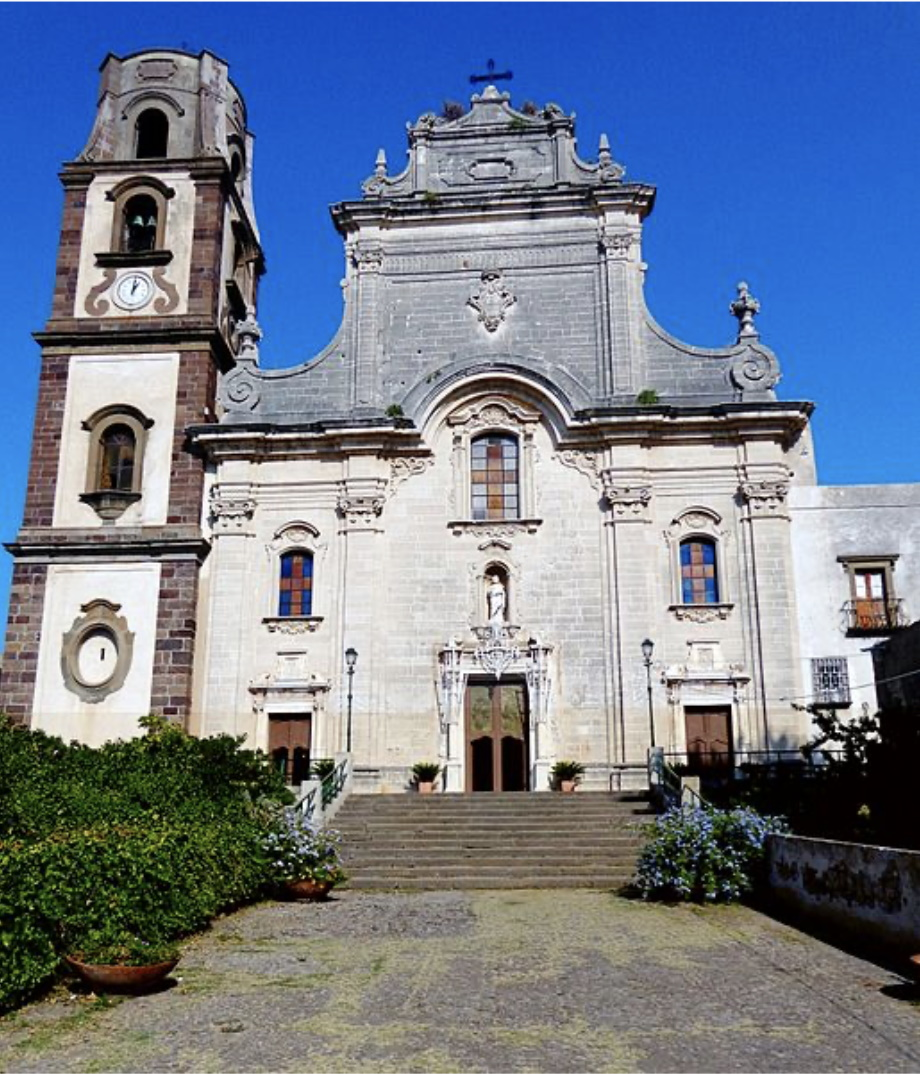
\includegraphics[width=0.8\linewidth]{san_bartolomeo}
	\caption{Basilca di San Bartolomeo}
	\label{fig:san_bartolomeo}
\end{figure}
 
A nord dell'isola, è possibile visitare le cave di pietra pomice che sovrastano il mare e creano contrasti cromatici mozzafiato; il sito è divenuto Patrimonio dell'Umanità tutelato e sovvenzionato dall'Unesco perché rimanga immutato.
Un sito di particolare interesse naturalistico è l'area marina di Punta Castagna che  si trova a nord est di Lipari ed è un fondale sabbioso di circa 15-40 metri. 

Data, quindi la grande presenza di siti archeologici e di numerose aree soggette a ricerche di diverso tipo, le attività edilizie comportano molto spesso un rischio dal punto di vista archeologico, in particolare nelle aree quali: Mendolita (zona in cui sono state rinvenute delle necropoli), Piano Conte, terreni lungo la strada tra San Calogero e Piano Corte, Castellaro Vecchio (dove vi furono insediamenti preistorici). Altre aree caratterizzate come potenzialmente archeologiche sono Quattropiani e Monte Giardina.


\subsubsection{Diritto fondiario}
Il territorio dell'isola di Lipari si estende su una porzione dell'isola pari a circa i 2/3 della superficie complessiva, ovvero \(\SI{2369}{\ettari}\) su \(\SI{3760}{\ettari}\). Nel territorio dell'isola, e su quello delle altre cinque isole amministrativamente costituenti il comune di Lipari, è stata istituita la Zona di Protezione Speciale "Arcipelago delle Eolie - area marina e terrestre" e sono in avanzato stato di definizione le procedure, ai sensi dell'art.4 della L.R.14/88, per l'istituzione di una nuova R.N.O. (Riserva Naturale Orientata) denominata "Isola di Lipari", già inserita nel Piano Regionale dei Parchi e delle Riserve. Inoltre, un'ampia porzione del suo territorio, prevalentemente nella parte occidentale dell'isola, seppur suddivisa in una zona di tutela propriamente detta e una zona di pre-tutela, è stata individuata quale area di interesse dall'UNESCO ai fini dell'iscrizione alla "World Heritage List" (WHL), ovvero candidata ad entrare nella lista del patrimonio mondiale dell'umanità, gestita dall' UNESCO. 

\subsubsection{Produzione e Consumi energetici}
Dalla scheda tecnica energetica di Lipari si può osservare che la fonte principale di alimentazione è il gruppo elettrogeno diesel. La produzione elettrica tramite fonti fossili è ancora molto alta rispetto alla potenza prodotta da fonti rinnovabili che copre solo l'\(\SI{1}{\percent}\) del fabbisogno energetico dell'isola. Si può osservare che, per quanto riguarda l'energia eolica, non sono state installate ancora tecnologie che sfruttano il vento per produrre energia elettrica, principalmente per ragioni di salvaguardia ambientale e per la presenza di politiche paesaggistiche rigide. Per quanto concerne il fotovoltaico invece, Lipari ha complessivamente una potenza installata di 508,89 kW, cifra irrisoria se confrontata ai consumi annui dell'isola.

Purtroppo Lipari è stata anche teatro di uno spiacevole episodio legato all'impianto fotovoltaico realizzato a Monte Sant'Angelo, il quale vantava il record per estensione tra tutte le isole minori del Mediterraneo. Con una potenza installata di \(\SI{1120}{\kW}\), l'impianto serviva a fornire oltre il \(\SI{20}{\percent}\) dell'energia necessaria a desalinizzare l'acqua, limitando così l'importazione di olio combustibile di circa 3 volte. Le circostanze però vollero che la sua realizzazione non fu mai completata, comportando uno spreco di circa 31 milioni di euro stanziati per abbattere l'emergenza idrica del paese. Un aumento della produzione da FER potrebbe permettere alle cisterne di stoccaggio di accumulare più acqua potabile, ottenuta con l'energia in eccesso da fonti rinnovabili durante la stagione invernale, al fine di coprire l'aumento di domanda che si verifica durante la stagione turistica. Gli impianti di dissalazione sono uno strumento fondamentale per Lipari in quanto rendono l'isola indipendente dal trasporto di acqua dalla terraferma e, inoltre, la combinazione con impianti di produzione di energia da fonti rinnovabili renderebbe possibile produrre acqua dolce localmente riducendo drasticamente le emissioni.

\begin{figure}[ht]\centering
	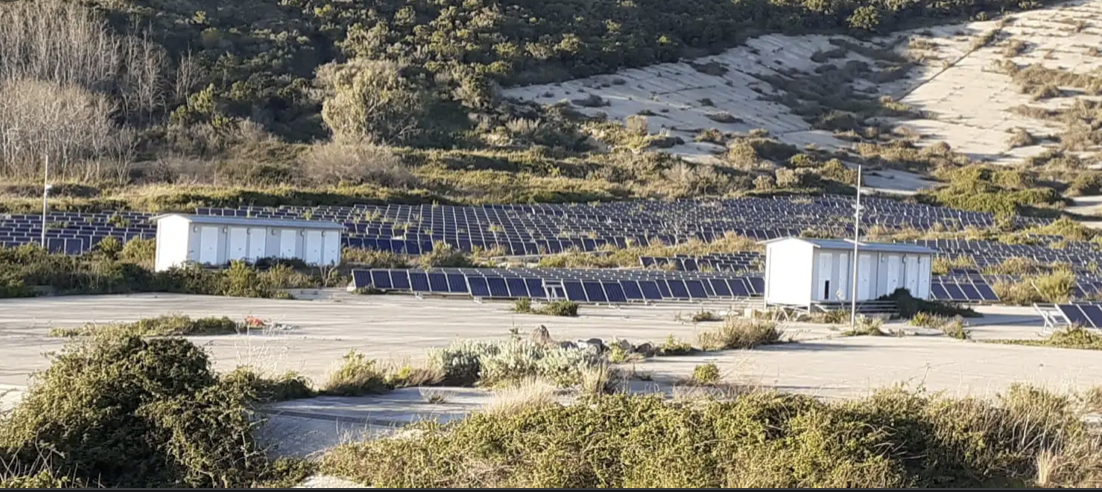
\includegraphics[width=0.8\linewidth]{lipari_solar_farm}
	\caption{Parco solare di Monte Sant'Angelo, Lipari}
	\label{fig:lipari_solar_farm}
\end{figure}

Continuando il discorso sulle fonti rinnovabili già presenti sull'isola, si fa largo anche una possibile introduzione di tecnologie che sfruttano il moto ondoso per produrre energia. I sistemi cosiddetti 'a colonna d'acqua oscillante' (Oscillating water column - Owc) sono dispositivi per la produzione di energia dal moto ondoso costituiti da una struttura di cemento o acciaio, parzialmente sommersa, con una camera aperta al di sotto della superficie dell'acqua al cui interno rimane intrappolata l'aria che si trova al di sopra dell'acqua. Il moto oscillatorio dell'acqua all'interno dell'apparato, prodotto dal moto ondoso, crea un flusso d'aria che aziona una turbina accoppiata ad un generatore elettrico. Il sistema, realizzato specificamente per le onde del Mar Mediterraneo, si innesca anche con onde basse, garantendo un'alta efficienza, garantendo attività per gran parte della giornata. Sono stati già testati due prototipi, nel dicembre del 2019 sul molo di Marina Corta di Lipari, la cui energia ricavata è stata utilizzata per alimentare i lampioni della banchina. 
Annualmente sull'isola di Lipari vengono consumati \(\SI{34.8}{\GWh}\) \cite{BandoLega} di energia.


\subsubsection{Produttività e Disponibilità di Tecnologie FER}
Analizzando la produttività delle tecnologie a nostra disposizione, si ottengono i seguenti CF medi:

\begin{table}[H]
	\caption{CF Medi annuali per Lipari}
	\centering
	\begin{tabular}{llc}
		\toprule
		Tecnologia   & CF \\
		\midrule
		Solare       & \(\SI{13.48}{\percent}\)         \\
		Eolico Offshore Palificato & \(\SI{17.40}{\percent}\)          \\
		WEC          & \(\SI{9.81}{\percent}\)         \\
		\bottomrule
	\end{tabular}
	\label{tab:lipari_cf}
\end{table}

È subito evidente che il solare sarà la tecnologia dominante per quest'isola, sia perché ha i suoi picchi di produzione in estate, durante la stagione turistica, quando è registrato il maggior consumo di energia, sia per la sua alta produttività rispetto al costo.

\begin{figure}[H]\centering
	\begin{tikzpicture}
		\begin{axis}[ yshift = 1cm,
				% grid=both,
				axis lines = left,
				xlabel = {Mese},
				ylabel = {CF Medio [\%]},
				ybar interval,
				ymax=0.3,
				ymin=0,
				xmin=0,
				xmax=13,
				width=0.8\linewidth,
				% area style,
			]
			\addplot+[ybar interval, mark=no] table [
				x=month,
				y=cf,
				col sep=comma
			] {PlotsData/lipari_solar_monthly.csv};
		\end{axis}
	\end{tikzpicture}
	\caption{Produzione di solare media per ogni mese dell'anno nell'isola di Lipari}
	\label{fig:monthly_solar_lipari}
\end{figure}


\begin{figure}[ht]\centering
	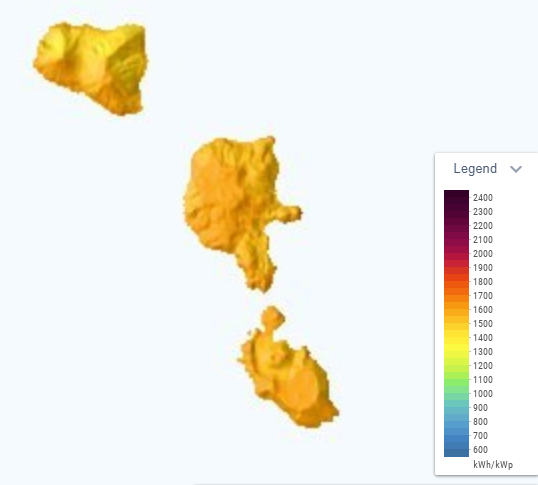
\includegraphics[width=0.8\linewidth]{lipari_solar}
	\caption{Mappa dell'irradiazione solare media di Lipari, da Global Solar Atlas}
	\label{fig:lipari_solar}
\end{figure}

Inoltre, si può notare come, nonostante il WEC non sia molto produttivo, incontra un ambiente relativamente mite nell'isola, che potrebbe essere utile per la ricerca e la raccolta di dati per potenziali futuri innovamenti della tecnologia.

Per quanto riguarda l'eolico, Lipari e le zone limitrofe sono molto poco ventose, quindi la tecnologia ha uno scopo molto limitato. 
Tuttavia, potrebbe rivelarsi utile installare qualche turbina a scopo di coprire i momenti in cui la produzione del solare è piuttosto limitata, come nei mesi invernali.

\subsubsection{Mercato energetico}
Lipari, essendo un'isola non interconnessa, deve provvedere alla produzione di energia sul suo territorio. Utilizza principalmente gasolio che viene importato tramite navi cisterna, con inevitabili rischi ambientali connessi. La conformazione stessa dell'isola e le avversità climatiche, poi, non rendono agevole la distribuzione e lo stoccaggio del carburante. Se già dal punto di vista del rendimento, una centrale a gasolio è molto meno efficiente di una centrale a gas, la spesa aumenta notevolmente considerando che al costo dell'energia vada sommato quello del trasporto. Non è un caso, infatti, se sulla terraferma la produzione di energia costi 3 volte meno rispetto a quanto ammonta per l'isola. 

Ragioni di equità sociale hanno tuttavia attenuato, fino ad annullarlo, il divario di prezzi dell'elettricità nelle isole minori rispetto a quelli nazionali: nonostante le condizioni territoriali siano profondamente diverse, gli abitanti delle isole minori pagano l'elettricità quanto quelli sulla terraferma. La compensazione tra i maggiori costi sostenuti dalle Aziende non coperti dai ricavi derivanti dalla vendita dell'energia elettrica è effettuata dalla Cassa per i Servizi energetici ambientali (CSEA). Questa spesa in più è sostenuta da ciascun consumatore che, pagando la bolletta dell'elettricità, in parte sta coprendo le spese per la distribuzione di energia elettrica nelle isole. Nel 2019 si è stimato che circa lo \(\SI{0.7}{\percent}\) della spesa media di un consumatore in energia elettrica era un contributo per diminuire i prezzi dell'energia nelle isole. 

Al fine di risolvere questa condizione di svantaggio delle isole minori non interconnesse, una possibilità può essere quella di connettere le isole alla rete elettrica nazionale, ciò però comporterebbe spese elevatissime per le infrastrutture da realizzare per rifornire un numero comunque esiguo di abitanti (a fronte delle elevate spese). A Lipari, così come anche in altre isole minori non interconnesse, un'ulteriore difficoltà è legata all'alta variabilità della domanda elettrica causata dalle grandi variazioni demografiche dovute soprattutto al turismo. 

Un'altra problematica di rilievo è che la separazione fisica determina una gestione indipendente delle reti, favorendo monopoli della produzione e della distribuzione di energia con ricadute economiche e ambientali. A tal proposito Lipari, a differenza della maggior parte delle isole minori non interconnesse italiane, non è gestita da Enel, ma da una società locale denominata Società Elettrica Liparese (SEL). 


\subsection{Contesto socio-culturale}
\subsubsection{Storia coloniale, decoloniale, post-coloniale.}
La storia di Lipari è una vicenda millenaria che ebbe inizio con le popolazioni del paleolitico superiore quando, secondo quanto si tramanda, qualche flotta attraversò il breve tratto di mare che separa Capo Milazzo dalle isole Eolie (tratto lungo poco più di 20 chilometri) e iniziò la loro colonizzazione. 
E' però solo a partire dal Neolitico che si ha la conclamata certezza della presenza della cultura agricola, importata da popoli che approdarono sull'isola portando una civiltà di gran lunga più sviluppata rispetto a quella delle popolazioni che vi avevano abitato fino a quel momento. Questo fervore coloniale è giustificato dalla presenza di tante materie prime di interesse per civiltà tecnologicamente più avanzate, in particolare il notevole uso dell'ossidiana. Le popolazioni insediate non usavano più le grotte come abitazioni, ma costruivano vere e proprie capanne, addensandosi in piccoli villaggi spesso fortificati. I primi reperti storici di Lipari sono stati ritrovati nella zona del "Castellaro Vecchio" presso la frazione di Quattropani, risalenti al IV millennio a.C., quando già in Sicilia queste ceramiche si trovavano nella loro fase evoluta. 

L'avvento della metallotecnica comportò due cambiamenti radicali per Lipari e tutte le Eolie: il primo fu la sostituzione dell'ossidiana con il bronzo, più facilmente lavorabile, meno fragile e non dipendente da una singola fonte di approvvigionamento; il secondo fu il miglioramento della marineria, dotata di navi più moderne che consentirono di intraprendere navigazioni più lunghe e non più legate ai percorsi costieri o limitate agli spostamenti a vista. Grazie alle sviluppate tecniche di navigazione, alla conformazione dell'arcipelago e alla sua posizione geografica centrale nel Mediterraneo, l'isola assunse una posizione preponderante nel commercio dello stagno proveniente dalla lontanissima Cornovaglia. 

Con l'avvento dei re italici, iniziò un'epoca di guerre e di paure che trasformò completamente l'economia e la stessa popolazione. A ciò si aggiunsero le eruzioni vulcaniche che provocarono una distruzione completa dei villaggi. Questo Medioevo ante litteram durò circa cinque secoli sino all'avvento della colonizzazione greca che nel 580 a.C. si impegnò nella ricostruzione dell'acropoli di Lipari. I greci erano molto attratti dall'isola per due motivi principali: il primo, prettamente economico, fu la presenza nell'isola di allume, utilizzato sin dall'antichità come fissante per colori, elemento basilare nella tintura delle stoffe; il secondo motivo, di carattere politico, fu la combinazione dell'eccellente capacità marinaresca dei greci con la posizione strategica dell'arcipelago al fine di contrastare la pirateria. Tutto ciò durò fino al III secolo a.C. quando, a causa delle guerre puniche, si concluse il dominio della Grecia, e l'isola passò sotto il controllo di Roma, perdendo nuovamente il suo ruolo centrale. 

ll II e I secolo a.C. furono caratterizzati da numerosissime eruzioni vulcaniche. Con l'avvento dell'imperatore Ottaviano, il primo periodo dell'Impero fu di assoluta tranquillità per tutta la Sicilia e per Lipari in particolare. 

Di rilievo fu, nei secoli a venire, l'influenza cristiana, la quale riecheggia ancora oggi nell'isola. La storia dell'isola ruota attorno alle vicende di Bartolomeo apostolo, morto decapitato in Albania negli anni delle rappresaglie contro i cristiani. La comunità in fuga raccolse il sarcofago con il corpo e si allontanò via mare, approdando dopo una violenta tempesta sulle coste di Lipari. La popolazione liparese che, per la sua posizione defilata, non aveva subito persecuzioni importanti, fu ben lieta di accogliere nella sua terra il corpo di un santo. Il sarcofago fu così portato nella zona che in quegli anni ospitava i raduni della comunità cristiana, subito fuori del paese dove oggi si può osservare la chiesa dedicata a San Bartolo extra moenia. Con la legalizzazione della fede cristiana, le chiese divennero cattedrali ed anche a Lipari la chiesa si spostò nel centro della città portando con sé anche le reliquie del santo. 

A san Bartolomeo si aggiunse, nel periodo delle rappresaglie barbariche, anche San Calogero che, stabilitosi in una zona impervia nella parte occidentale dell'isola (nei pressi dell'attuale frazione di Pianoconte), rimise in funzione le antiche terme di fattura greco-romana, consentendo alla gente del luogo di sfruttarne le doti terapeutiche. Da questo momento in poi non si hanno più notizie fino al 1084 quando l'isola entra a far parte del regno di Sicilia grazie a Ruggero, il quale fece costruire un monastero benedettino che potesse attirare attorno a sé un nucleo abitativo sufficientemente consistente per l'eventuale difesa delle isole, donando terre da coltivare ai contadini.

\subsubsection{Storia culturale, sociale, politica.}
Le tradizioni culturali dell'isola sono profondamente legate alla sua storia coloniale. Notevole fu l'influenza dei greci, sia negli aspetti più culturali quali l'importazione delle pratiche mercantili, della lavorazione delle ceramiche, sia nella costituzione politico-sociale della città. In quest'epoca fu impiantato il modello della polis, la quale, definita dalle mura difensive, vedeva la città suddivisa tra la sua parte alta, l'acropoli, dove si trovavano i templi ed edifici pubblici, l'agorà, luogo dedicato ai mercati e alle assemblee e la parte bassa, dove viveva la maggior parte della popolazione. Lipari, per la sua conformazione territoriale, si rivelò perfettamente adatta all'inserimento di questo modello socio-politico.

Di notevole importanza da molteplici punti di vista risultò poi l'avvento del cristianesimo, che definì la  nascita di quella tradizione religiosa che ancora oggi è al centro dell'isola. Infatti sono numerose le manifestazioni sacre nella tradizione dell'isola che si tramandano ancora oggi  e che la rendono celebre e famosa. Le celebrazioni più importanti si tengono in onore del patrono dell'isola, San Bartolomeo: la manifestazione dura molteplici giorni con concerti e mercatini all'aperto, culminando poi il 24 agosto con la processione e giochi pirotecnici. Accanto a ciò vi sono la processione del Venerdì Santo, dove tutte le confraternite indossano gli abiti tipici, portando per le vie del paese le sacre statue chiamate varette, seguita da quella della Domenica di Pasqua, la quale vede un incrocio del corteo dedicato alla Madonna con quello dedicato a Gesù nella piazzetta di Marina Corta. 

Inoltre, in campo sportivo, si organizza ogni estate la "Manifestazione sportiva dello Judo", evento della durata di 3 giorni, dove accorrono ragazzi da tutta l'Italia ed anche dall'estero. Sempre in questo periodo si tiene nella baia di Marina Lunga, una sfilata di barche pittoresche che procedono per tutta la baia. 
Il dialetto di Lipari, è comune a tutte le isole Eolie, ed è la variante della lingua siciliana parlata nell'isola maggiore. Esso riflette a pieno tutte le variazioni culturali e sociali che si sono succedute nel tempo. Infatti risente dell'influenza di diversi nuclei dialettali come quello di Milazzo, Messina e Barcellona. Sorprendente è però anche l'assonanza dei detti tipici del posto con quelli laziali e con il sardo. 

Ma la contaminazione preponderante fu introdotta inconsapevolmente, nel '900, quando un gruppo di pescatori siciliani residenti in diversi centri abitati delle coste orientali dell'isola, si trasferì a Lipari. Questo provocò un fiorente scambio culturale e lessicale tra i siciliani e gli abitanti di Lipari.

\paragraph*{Contesto politico e ambientale attuale.}
L'ingegnere Alex Sorokin, titolare dell'Interenergy con sede a Roma dal 1996 si è occupato inizialmente di un'analisi panoramica di tutte le isole minori italiane per conto di Enel; successivamente nel 2002 è passato ad uno studio esclusivo su Lipari e Salina dimostrando che, con un passaggio graduale alle fonti rinnovabili che comprendevano solare, eolico e geotermico, non solo i costi sarebbero diminuiti, ma si sarebbe anche ottenuto anche un impatto positivo sulla visibilità e sulla qualità della vita nell'isola. 

La grande difficoltà che sussiste a Lipari, come affermò il  sindaco Marco Giorgianni nel 2013, riguardava motivazioni legate a innumerevoli leggi, di cui la maggior parte per la tutela paesaggistica; infatti a Lipari non era permesso posizionare sui tetti neanche un pannello solare termico. Ora, con una modifica consistente al PRG (Piano Regolatore Generale) per le isole Eolie, si è eliminato questo vincolo sui pannelli solari.

Il 14 febbraio 2017 il ministero ha promulgato degli obiettivi minimi di sviluppo delle fonti rinnovabili nelle isole non interconnesse da perseguire entro il 2020 quali: 
\begin{itemize}
	\item installazione, presso utenze domestiche e non domestiche, di sistemi con pannelli solari termici per la copertura dei consumi di acqua calda o per il solar cooling. Concorre a tale obiettivo anche l'installazione, esclusivamente in sostituzione di scaldacqua elettrici, di pompe di calore dedicate alla sola produzione di acqua calda sanitaria;
	\item installazione di impianti di produzione di energia elettrica collegati alla rete elettrica isolana, alimentati dalle fonti rinnovabili disponibili localmente. I predetti impianti di produzione possono essere asserviti a specifiche utenze, ivi inclusa la ricarica di veicoli elettrici, con immissione parziale nella rete elettrica, ovvero possono immettere in rete tutta l'energia elettrica prodotta.
\end{itemize}

In più per ogni isola sono stati stabiliti dei limiti minimi che nel caso di Lipari sono:
\begin{enumerate}
	\item obiettivo potenza FER di 2110  kW elettrici;
	\item obiettivo superfici solari termiche di \(\SI{2520}{\m\squared}\);
	\item produzione annua convenzionale di \(\SI{34800}{\MWh}\) elettrici.
\end{enumerate}

Attualmente invece, il  sostentamento energetico  avviene ancora principalmente tramite centrali termoelettriche a gasolio e questo denota come gli obiettivi minimi imposti dal Ministero non siano stati raggiunti. A Lipari si stima di essere arrivati, con le rinnovabili, a coprire circa l'\(\SI{1}{\percent}\) del fabbisogno energetico.  
% TODO: Inserire rapporto isole sostenibili 2021.

Per questo, per incentivare, nel 2020, il Ministero dell'Ambiente e della Tutela del Territorio e del Mare, ha finanziato diversi progetti per 4 isole italiane, tra cui Lipari, i quali hanno come obiettivo quello di offrire interventi di efficienza energetica, mobilità sostenibile e adattamento agli impianti ai cambiamenti climatici nelle isole minori. 

Il progetto dedicato a Lipari prende il nome di MEGALITERA "Mobilità elettrica per lo spostamento giornalieri a Lipari e interventi tecnici di efficientamento della rete idrica attuale". Il tutto, prevede di migliorare i servizi essenziali offerti alla cittadinanza impattando da un punto di vista energetico con una riduzione dei consumi e dei costi. Questo sarebbe da applicare prevalentemente nel campo dei trasporti e della mobilità, ma anche nell'ambito della rete idrica evitando sprechi di energia per il funzionamento dei dissalatori. 

Il bando "Aree marine protette per il clima", analogamente al progetto "Parchi per il clima" che è alla sua terza edizione, prevede finanziamenti a interventi di efficienza energetica del patrimonio immobiliare pubblico nella disponibilità dell'area marina protetta e a interventi per la realizzazione di servizi e infrastrutture di mobilità sostenibile terrestre e marina.
In più il comune ha deciso di aderire all'iniziativa della Comunità Europea denominata "Covenant of Mayor for Climate and Energy", la quale prevede la redazione di un Piano di Azione per l'energia sostenibile da attuare entro il 2030 con l'obiettivo di ridurre le emissioni del \(\SI{40}{\percent}\).

Il turismo può essere una fonte di rischio a livello ambientale e per questo la Legge 221/2015 ha istituito per i viaggiatori che approdano sulle Isole Minori l'obbligo di versare il contributo di sbarco, una forma di tassazione ambientale in sostituzione all'imposta di soggiorno normalmente applicata dai Comuni. I proventi dovranno essere destinati a finanziare e sostenere la raccolta e lo smaltimento dei rifiuti, il recupero e la salvaguardia ambientale. 


\subsection{Modellazione energetica}
Introdurre energia rinnovabile nell'isola di Lipari presenta molte sfide, sia dovute alla geografia locale, sia dovute all'intero corpus di leggi che limita lo sviluppo di nuove tecnologie nell'isola.
Un'ottimizzazione non limitata del progetto in quest'isola produce i seguenti risultati, utilizzando turbine eoliche onshore:
\begin{table}[H]
	\caption{Progetto non limitato per Lipari}
	\centering
	\begin{tabular}{llc}
		\toprule
		Tecnologia   & Potenza/Capacità Installata \\
		\midrule
		Solare       & \(\SI{22.88}{\MW}\)         \\
		Eolico       & \(\SI{1.213}{\MW}\)          \\
		WEC          & \(\SI{0.000}{\MW}\)         \\
		Accumulatori & \(\SI{72.26}{\MWh}\)        \\
		\bottomrule
	\end{tabular}
	\label{tab:lipari_unbounded_1}
\end{table}

Questo progetto prevede di installare una quantità di solare non realistica, poiché sull'isola non vi è abbastanza spazio pianeggiante per una centrale di tali dimensioni, quindi, nonostante ciò permetterebbe all'energia annuale dell'isola di essere generata dalle rinnovabili per l'\(\SI{85.36}{\percent}\), si ritiene necessario cercare una soluzione più realistica.
Nel sito di Monte Sant'Angelo e, favorendo l'installazione sui tetti sia di edifici pubblici, sia incentivando i privati, è stimata un'installazione di solare pari circa a \(\SI{12.00}{\MW}\). Inserendo questa limitazione, si arriva ad un piano come quello descritto in tabella.

\begin{table}[H]
	\caption{Progetto limitato per Lipari}
	\centering
	\begin{tabular}{llc}
		\toprule
		Tecnologia   & Potenza/Capacità Installata \\
		\midrule
		Solare       & \(\SI{12.00}{\MW}\)         \\
		Eolico       & \(\SI{5.00}{\MW}\)          \\
		WEC          & \(\SI{1.00}{\MW}\)         \\
		Accumulatori & \(\SI{45.08}{\MWh}\)        \\
		\bottomrule
	\end{tabular}
	\label{tab:lipari_bounded}
\end{table}

Una volta limitato il solare, l'algoritmo usato per l'ottimizzazione suggerisce l'aggiunta di una turbina eolica da \(\SI{5.00}{\MW}\), per rimpiazzare la potenza di solare non installabile.
Questa turbina verrebbe collocata offshore, nel mare ad ovest della costa, in modo da non intralciare le rotte commerciali verso l'isola, e rispettare le rigide leggi sull'eolico locali.
Idealmente, questa turbina potrebbe essere parte di un parco eolico più esteso, tale da fornire energia all'intero arcipelago delle Eolie, oltre che al resto della Sicilia.
Questa soluzione sfrutterebbe le rinnovabili per il \(\SI{67.24}{\percent}\) dell'energia annua.

Una nota da fare è che il WEC installato non fa parte del risultato dell'algoritmo.
Infatti, l'algoritmo consiglia di non utilizzare proprio tale tecnologia, ma se ne ritiene utile l'installazione sia per aumentare l'affidabilità del sistema, che potrebbe così affidarsi a più tecnologie, sia per poter accumulare più dati per la ricerca, in modo da produrre tecnologie WEC più prestanti nel futuro.

In questo modo, l'energia prodotta e usata mensilmente si distribuisce come in figura \ref{fig:monthly_consumption_lipari}. Il LCOE stimato è \(\SI{0.177}{\EUR\per\kWh}\)

\begin{figure*}[ht]\centering
	\begin{tikzpicture}
		\begin{axis}[ 
				% yshift = 1cm,
				% axis lines = left,
				yshift = -1cm,
				xlabel = {Mese},
				ylabel = {Consumo [GWh]},
				ybar stacked,
				% ybar legend,
				% ymax=0.3,
				% ymin=0,
				% xmin=0,
				% xmax=13,
				% xmin=1,
				% xmax=12,
				date coordinates in=x,
				xtick=data,
				xticklabel={\pgfcalendar{tickcal}{\tick}{\tick}{\pgfcalendarshorthand{m}{.}}},
				width=0.8\linewidth,
				legend style={at={(0.5,-0.13)},
                    anchor=north,legend columns=-1},
				% area style,
			]

			\addplot+[ybar, mark=no, black, fill=RedOrange] table [
				x=month,
				y=solar,
				col sep=comma,
				y expr=\thisrow{solar}*1e-9,	
			] {PlotsData/lipari_consumption.csv};

			\addplot+[ybar, mark=no, black, fill=SeaGreen] table [
				x=month,
				y=wind,
				col sep=comma,
				y expr=\thisrow{wind}*1e-9,
			] {PlotsData/lipari_consumption.csv};

			\addplot+[ybar, mark=no, black, fill=NavyBlue] table [
				x=month,
				y=wec,
				col sep=comma,
				y expr=\thisrow{wec}*1e-9,
			] {PlotsData/lipari_consumption.csv};

			\addplot+[ybar, mark=no, black, fill=yellow] table [
				x=month,
				y=accumulator,
				col sep=comma,
				y expr=\thisrow{accumulator}*1e-9,
			] {PlotsData/lipari_consumption.csv};

			\addplot+[ybar, mark=no, black, fill=black] table [
				x=month,
				y=diesel,
				col sep=comma,
				y expr=\thisrow{diesel}*1e-9,
			] {PlotsData/lipari_consumption.csv};

			\legend{Solare, Eolico, Wec, Accumulatori, Diesel}
		\end{axis}
	\end{tikzpicture}
	\caption{Consumo mensile per tecnologia nell'isola di Lipari}
	\label{fig:monthly_consumption_lipari}
\end{figure*}

\subsection{Strategia di accesso al campo e posizionamento}
L'installazione degli impianti energetici appena descritti non può essere tuttavia decisa a priori, in quanto, oltre ai dati già raccolti, esistono tante altre informazioni che possono essere acquisite solo mediante l'accesso al campo e il contatto diretto con il luogo in esame e la sua popolazione. Senza di ciò sarebbe infatti impossibile conoscere tutta una serie di aspetti legati al territorio e alle leggi presenti, ma soprattutto alla volontà della popolazione residente e delle istituzioni. 

\subsubsection{Portatori di interesse (potere decisionale, influenza, obiettivi)}
Uno dei  principali stakeholders da tenere in considerazione e coinvolgere per la miglior riuscita del progetto è l'amministrazione comunale che, come si evince da diverse dichiarazioni rilasciate in passato,  è ben attenta all'evoluzione dell'isola. Anche il comune sarà un attore molto importante nel progetto soprattutto per la richiesta di rimettere in uso l'impianto fotovoltaico abbandonato presso il monte St. Angelo per alimentare il fabbisogno energetico dell'isola.  

Un altro interprete di grande rilevanza risulta la società locale energetica SEL SNC Lipari, con il loro aiuto si prevede di avere maggiori dati sui consumi e sui costi, ma soprattutto finanziatori certi per l'evoluzione del progetto.  Le società edilizie avranno un loro ruolo di interesse, in quanto, data la difficoltà a trovare un territorio idoneo alla installazione di pannelli solari, si prevede una collaborazione con il mondo delle costruzioni, con incentivi sulle bollette per i cittadini nel caso in cui scelgano di acquistare abitazioni con pannelli solari, oppure di installarne nuovi sulle loro abitazioni. In aggiunta a ciò, è molto importante considerare anche le leghe ambiente della zona, come la FLAI (federazione lavoratori agro industria) i quali oltre ad essere molto attivi nel rispetto dell'ambiente, si occupano principalmente di preservare i diritti degli agricoltori, una delle principali fonti di sostentamento dell'isola. 

In ultima istanza, va considerata la partecipazione attiva della popolazione locale. Infatti essa rappresenta l'istituzione non dichiarata  di maggior importanza per l'approvazione di tutto il progetto. Ciò, tuttavia, non dovrebbe rappresentare un problema, almeno in fase di raccolta di dati sul luogo, in quanto l'isola è frequentemente adibita a studi di ogni genere, date le sue caratteristiche peculiari in molteplici ambiti.

\subsubsection{Legittimità e riconoscimento (pratiche, comportamenti e protocolli)}
Il territorio di Lipari presenta una serie di norme restrittive sull'utilizzo dei terreni in quanto esistono leggi per preservare al massimo il paesaggio, ma soprattutto le tradizioni e la popolazione residente.  

Nel documento "Approvazione del Piano territoriale paesistico dell'arcipelago delle Isole Eolie" del 23 febbraio 2001, redatto dalla regione Sicilia, nell'articolo 9 si sanciscono le tipologie di interventi compatibili all'interno delle attività dell'isola. A Lipari è possibile effettuare ricerca scientifica di monitoraggio, l'isola è sempre stata infatti oggetto di studio, per esempio per quanto riguarda la tettonica delle placche, per la geodinamica del Mar Tirreno e per la vulcanologia. Ciò comporta una forte presenza sul territorio di università e istituti di ricerca, ed è nell'interesse della stessa amministrazione comunale facilitare l'esecuzione di tali iniziative e attività.
Inoltre, con l'articolo 10,  viene data la possibilità di recupero edilizio conservativo, che darebbe l'opportunità di sfruttare, adattandolo ai nuovi standard, l'impianto fotovoltaico sul Monte St. Angelo, già installato, ma mai entrato in funzione. 

Per quanto concerne invece le relazioni di fiducia da stabilire con i cittadini, si segue il modello del protocollo di Otago (2011), il quale riconosce la non uniformità delle convenzioni, dei valori e dei costumi nei diversi territori. A questo si aggiungono gli Standard di Ricerca (KULANA NOI'I), la cui idea nasce (così come per il protocollo di Otago) per fornire indicazioni sul rapporto ricercatore-popolazione per le isole oceaniche, ma che possono essere facilmente adattati a tutti i territori insulari oggetto di ricerca. Il documento comprende 8 pratiche suggerite, per dare standard di ricerca collaborativa al fine di creare relazioni e collaborazioni vantaggiose da entrambi i lati. Il tutto va fatto attraverso un dialogo costruito con la popolazione locale, dove si mostrano chiaramente quali sono gli obiettivi da perseguire, le evidenze che portano all'analisi del territorio per gli oggetti in esame e, ovviamente, come si intende procedere tenendo sempre aggiornati tutti gli interessati su eventuali variazioni rispetto al programma di partenza. Inoltre, uno studio così specifico e poco generalizzabile può essere arricchito attraverso moduli da far compilare ai cittadini, così da avere anche la loro visione dei problemi ed eventuali finestre innovative che da non residente nelle zone di interesse, non si può pretendere di avere. 

Tutto ciò, però, deve essere sempre guidato dal massimo rispetto per gli usi ed i costumi della popolazione locale, e soprattutto per il territorio. Per questo, nel decreto sopra citato nell'articolo 37, si tiene ancora una volta a precisare "La disciplina degli usi civici è espressamente finalizzata alla conservazione delle risorse naturali attraverso un uso collettivo che sia compatibile con la loro conservazione e trasmissione (senza la quale l'uso civico verrebbe a mancare)."


\subsection{Conclusioni}
\subsubsection{Limiti e opportunità}

L'isola di Lipari è l'isola maggiore dell'arcipelago eoliano con la sua superficie di 37,6 km2 e il più alto tasso di turismo di tutto l'arcipelago. L'analisi morfologica e territoriale condotta denota alcune peculiarità dell'isola: le coste sono prevalentemente alte e frastagliate e anche l'entroterra ha forme molto irregolari. Queste caratteristiche sono state oggetto di attente valutazioni nella fase di scelta dei siti di installazione. Particolare attenzione è stata posta ai progetti già avviati nell'isola come il parco fotovoltaico nei pressi del monte Sant'Angelo. 

Un aspetto importante riguarda lo studio dei flussi turistici soprattutto nelle stagioni estive in cui il consumo energetico medio aumenta a causa del maggior numero di utenze; la variabilità così accentuata della domanda energetica durante l'anno mette a dura prova i modelli energetici. Proprio per questo motivo sono state valutate tutta una serie di strategie per massimizzare la produzione energetica nelle stagioni più calde. Il parco fotovoltaico già presente, oltre che non essere attivo, risulta insufficiente a soddisfare i requisiti energetici dell'isola. 

Parallelamente alle indagini fatte sugli impianti già presenti è necessario ricordare tutte le problematiche legate all'aspetto socio-politico: il territorio di Lipari presenta una serie di normative che regolamentano l'uso e la destinazione delle aree, tramite la protezione civile e la guardia costiera si osserva la salvaguardia delle aree protette (ZPS/SIC). Per ogni isola inoltre sono stati stabiliti dei limiti minimi di sviluppo che tutt'oggi non risultano soddisfatti, per questo motivo sono stati stanziati fondi europei (PNRR) e finanziati progetti come quello del Ministero dell'Ambiente e della Tutela del Territorio e del Mare dove quattro isole Italiane, tra cui Lipari, vengono finanziate allo scopo di offrire interventi di efficienza energetica.


\subsubsection{Analisi delle opzioni}

I risultati proposti nella fase di modellazione energetica sono frutto di continue rivalutazioni mirate al perfezionamento del progetto, non escludendo la necessità di scendere a compromessi dovuti ad aspetti caratteristici di Lipari. Un esempio è dato dal fatto che le limitazioni morfologiche non considerate in prima analisi dall'algoritmo avevano suggerito una potenza installabile di fotovoltaico pari a 22,88 MW, una quantità nettamente superiore a quella realisticamente installabile a causa della bassa presenza di superficie pianeggiante, per questo motivo si è scelto di analizzare alternative diverse. Grazie alla versatilità dell'algoritmo genetico è stato possibile andare a limitare il parametro di potenza da energia solare.

Ciò ha portato, nonostante la posizione geografica di Lipari ne caratterizzi una risorsa di vento limitata, che si traduce in un CF piuttosto basso per l'eolico, alla necessità di installare una turbina per raggiungere l'indipendenza dalle fonti fossili. La presenza in gran parte dell'isola di coste alte e frastagliate e le diverse leggi sulla salvaguardia del territorio limitano però gli spazi per l'installazione. La scelta sul posizionamento della tecnologia, quindi, limitata sia dalla morfologia dell'isola, sia da una serie di fattori come l'elevato traffico marino nella zona sud-est dell'isola, ricade nella zona di mare a ovest dell'isola. 
Per quanto concerne il WEC,  pur avendo l'LCOE più alto tra quelli delle tecnologie analizzate, rappresenterebbe un importante strumento per la raccolta di dati e l'aggiornamento di impianti simili, in modo da contribuire nel tempo alla consolidazione di tali sistemi ancora in fase di sviluppo.



% ==================
% COMPARAZIONE
% ==================

\section{Comparazione}
Le isole sono il laboratorio ideale per affrontare, e vincere, le sfide ambientali più urgenti e importanti che il Mondo ha di fronte.
Riprodurre un modello energetico dipendente al \(\SI{100}{\percent}\) da fonti rinnovabili è uno degli obiettivi dell'accordo di Parigi (2015). Le isole, oltre a fornire dei casi studio semplificati per la modellizzazione energetica, ci permettono di mettere in chiaro i problemi e i punti di forza di tali modelli e di estenderli a casi sempre più generali; nelle isole inoltre il costo di produzione e distribuzione dell'energia è amplificato rispetto alla terraferma e questo rende le tecnologie rinnovabili di per sé già consolidate ancora più competitive. Ogni isola rappresenta un caso studio diverso e, dal punto di vista sia antropologico sia ingegneristico, per ciascuna sarebbe necessario fare un discorso separato; nonostante ciò l'obiettivo è comune: da un lato soddisfare la domanda energetica  e gli obiettivi prefissati tramite un'attenta analisi delle tecnologie e una differenziazione delle stesse, dall'altro preservare la bellezza e la cultura di ogni isola ma soprattutto il benessere di ogni cittadino. Dal punto di vista dell'ecosostenibilità, avere uno sguardo sempre rivolto al futuro è un aspetto fondamentale: l'introduzione di tecnologie sempre più innovative nell'ambito del rinnovabile dovrebbe anche stimolare le nuove generazioni a crescere in un'ottica più green, concentrando sempre più l'attenzione sulla ricerca verde. 

Il confronto tra le due isole passa per più punti. L'obiettivo è quello di delineare un quadro delle due isole attraverso una serie di considerazioni che mettano in luce quali possano essere le opportunità e le criticità di ciascuna di esse di fronte a un progetto di rinnovamento energetico che prevede il passaggio dall'utilizzo di fonti fossili a quello di fonti rinnovabili.


\subsection{Differenze ambientali e territoriali}
Il primo aspetto che si prende in considerazione è quello ambientale e sociale. Le due isole, nonostante siano entrambe di origine vulcanica, hanno una morfologia del territorio piuttosto differente. Il territorio di Wallis infatti è lagunare con la presenza di altipiani nell'entroterra e di una zona costiera dove risiede la maggior parte della popolazione; è inoltre caratterizzato da numerosi laghi di origine vulcanica e dall'assenza di spiagge. Un elemento molto importante, poi, è la barriera corallina, la quale è messa a rischio dai cambiamenti climatici e, dal momento che da essa dipende la sopravvivenza di un intero ecosistema marino, la sua salvaguardia è fondamentale. Il territorio di Lipari invece è quello caratteristico della macchia mediterranea, caratterizzato inoltre dalla presenza di numerosi altipiani generati dall'intensa attività vulcanica presente sull'isola molti secoli fa. 
Queste differenze morfologiche evidenziano la necessità di operare una diversificazione sui percorsi da intraprendere per le due isole. A livello territoriale andrebbe rimarcata la politica adottata dalle due isole per preservare il territorio. 

Lipari è un territorio patrimonio dell'Unesco dal 2000 e gode di aree che sono protette tramite delle legislazioni previste dallo Stato Italiano e dall'Europa (ZPS, SIC). Sono numerosi infatti i siti protetti come quelli archeologici di epoca greco romana e le numerose aree naturali ad alta biodiversità. Sull'isola sono presenti enti di salvaguardia e tutela come la guardia forestale che si occupa della gestione delle riserve naturali.

Un discorso diverso va affrontato per Wallis, dove non ci sono vere e proprie normative che regolano la salvaguardia di determinate zone; è stato, infatti, adottato solo nel 2007 un codice ambientale atto a preservare il mantenimento della biodiversità di determinate aree geografiche; oltre a ciò si aggiunge un forte senso di rispetto per la natura da parte dei nativi, motivo per cui esistono molte aree apparentemente disponibili a progetti di installazione, in cui però non si possono realizzare attività scientifiche in quanto ritenute inviolabili. Un ruolo fondamentale è ricoperto dagli stakeholders e dalle assemblee cittadine che esprimono il potere decisionale e possono consentire la realizzazione del progetto. Inoltre è necessario ottenere il consenso del re e delle figure a capo dell'isola. Al fine di conoscere il contesto sociale e culturale da cui prende forma ogni progetto sul campo, gli antropologi hanno un ruolo determinante nello studio delle piccole società insulari; per realizzare un progetto ecosostenibile è necessario, infatti, comprendere le varie sfaccettature della società, avere la capacità di comprendere tutta una serie di informazioni non comunicate apertamente, ma attraverso il non detto, le metafore, gli stili di vita e i comportamenti socio-culturali ed etici che non appaiono subito chiari agli occhi dell'ospite e che prescindono da ogni forma di regola scritta o legge. 


\subsection{Differenze storico-legislativo-sociali}
Dal punto di vista storico e sociale possiamo estrapolare alcune informazioni utili per confrontare le diverse politiche energetiche adottabili. Wallis ha avuto una storia turbolenta con i coloni prima inglesi e poi francesi che approdarono sull'isola a partire dalla seconda metà del Settecento e il più delle volte i problemi scaturirono dal rapporto degli abitanti con il loro territorio. Se si vuole dunque modificare il territorio con interventi umani bisogna avere una reale coscienza delle usanze e abitudini del luogo. La popolazione di Wallis vive di un'economia prettamente agricola in cui lo scambio di mercato è praticamente assente e termini come "ricchezza" e "valuta" non sono concepiti. Questo dato importante mette in luce la distanza di Wallis da un'ottica di ragionamento e di pensiero tipica invece di paesi europei, o comunque completamente sviluppati, di cui Lipari fa parte. Qui le difficoltà sono principalmente legate alla protezione del paesaggio e una legislazione piuttosto rigida riguardo tutte le attività umane di modifica del territorio. Nonostante ciò si evidenzia un buon livello dell'isola di apertura verso la ricerca scientifica che ha visto Lipari al centro di molti studi negli ultimi anni.

Le modalità di approccio al campo decretate dal protocollo di Otago pensate per le isole oceaniche possono essere applicate anche alle isole mediterranee. Questo protocollo stila 8 punti in cui si afferma che ciascuna isola ha la sua cultura e le sue usanze e che, in particolare, nel realizzare un progetto e nello svolgere ricerca scientifica bisogna quanto più possibile coinvolgere la popolazione, per tenerla informata sul progetto stesso, su eventuali cambi di piano e cercare di apprendere dal popolo stesso tutte le criticità e opportunità.

\subsection{Differenze Energetiche}
Se da una parte bisogna riconoscere che un possibile intervento sull'isola possa avere delle conseguenze irreversibili sul suo territorio e sul paesaggio, dall'altro bisogna anche ricordare che queste isole dal punto di vista energetico sono molto lontane dall'autosufficienza e devono affidarsi a centrali termoelettriche che per produrre energia devono affrontare spese molto elevate. La mancanza di indipendenza energetica è quindi uno dei fattori che più spinge verso l'installazione di tecnologie che sfruttano fonti rinnovabili innovative.

Le due isole attualmente traggono la maggior parte del sostentamento energetico da generatori a diesel. Le tecnologie attualmente installate sono poco incoraggianti: a Wallis è presente un solo impianto fotovoltaico in grado di produrre \(\SI{128}{\kWp}\), la maggior parte dell'energia è prodotta nella centrale termoelettrica da \(\SI{6.78}{\MW}\) della società EEFW che gestisce l'equilibrio tra domanda e offerta energetica, non particolarmente influenzata dai flussi turistici dell'isola. L'obiettivo di sviluppo della società  è quello di implementare \(\SI{3}{\MW}\) di fotovoltaico nelle zone disponibili dell'isola. 

Sono stati trovati diversi siti potenzialmente utili all'installazione di tale tecnologia e presi in esame ai fini della modellazione energetica. Tramite l'impiego dell'algoritmo genetico usato per l'ottimizzazione, ed un successivo studio e analisi delle risorse, si evince una netta preferenza del fotovoltaico.

Lo studio effettuato permette una modellazione energetica quanto più attenta e integrativa ma soprattutto in grado di guardare al futuro e di fare proiezioni su scenari ambientali e socio-politici. Per questo motivo si sono aperte le porte anche ad altri scenari energetici meno competitivi ma comunque molto validi come l'eolico off-shore e il WEC. L'eolico off-shore presenta più che svantaggi diverse difficoltà dettate dalla conformazione lagunare dell'isola e dall'importantissima presenza della barriera corallina. Viene proposta una soluzione del tutto innovativa ed in fase di sviluppo che permetterebbe di coniugare l'efficienza dell'eolico off-shore alla salvaguardia della barriera corallina e dell'intero ecosistema che da essa dipende, sede di una vastissimo numero di specie marine. 

Il progetto per l'isola di Lipari presenta numerosi vantaggi sia in termini energetici sia in termini economici. Il parco fotovoltaico posto nelle vicinanze del monte Sant'Angelo costruito tra il 2014 e il 2015 con fondi regionali rappresenta un'enorme ricchezza, che a causa di cavilli burocratici e contenziosi si è trasformata in un disastro economico-ambientale. La centrale solare di Lipari da oltre 1 MW adesso si trova fuori uso in attesa di essere smaltita. Lo scopo originale di questo progetto era quello di supportare il funzionamento del nuovo dissalatore; secondo i calcoli sarebbe riuscito ad estrarre dalla radiazione solare circa il \(\SI{20}{\percent}\) dell'energia necessaria a desalinizzare l'acqua marina evitando l'importazione di una notevola quantità di olio combustibile. I gruppi elettrogeni presenti a Lipari tutti di proprietà della società elettrica liparese sono ormai datati e in confronto alle nuove centrali a combustibile fossile hanno dei rendimenti molto modesti, di circa il \(\SI{40}{\percent}\). Nella terraferma inoltre il costo della produzione energetica è di circa 3 volte minore rispetto alle isole dell'arcipelago eoliano e l'efficienza di tali centrali termoelettriche si affievolisce ancor di più col fatto che nella maggior parte delle case, ad eccezione degli esercizi commerciali, è presente un impianto elettrico datato; una casa vecchia  di 30 anni consuma ogni anno in media dai \(\SI{180}{\kWh\per\metre\squared}\) ai \(\SI{200}{\kWh\per\metre\squared}\) mentre una casa nuova può arrivare a consumare anche \(\SI{30}{\kWh\per\metre\squared}\); bisogna poi aggiungere che trattandosi di un isola l'approvvigionamento del combustibile come anche di molte altre risorse è molto meno agevole rispetto alla terraferma.

Il consumo energetico medio di Lipari si stima essere intorno ai \(\SI{22}{\MWh}\), valore che varia di molto in base alla stagione e ai flussi turistici annui.  
Il fotovoltaico su Lipari che al momento copre solo l'\(\SI{1}{\percent}\) del fabbisogno energetico, risulta, come nella precedente trattazione su Wallis, essere la soluzione più concreta ed efficace in termini di costo-beneficio, ipotesi confermata dal fatto che un progetto di solare abbia già preso vita. Un sostanziale punto di differenza tra le due isole è dettato dai flussi turistici annui, Lipari rappresenta una meta turistica ambita in Sicilia. I tassi turistici sono i più alti di tutto l'arcipelago delle Eolie: nel 2020, per esempio, si è registrata la presenza di 7800 nuovi arrivi e in Sicilia un aumento delle prenotazioni del \(\SI{420}{\percent}\). L' impennata delle presenze nei mesi caldi, come si evince dalla figura \ref{fig:monthly_consumption_lipari}, impatta notevolmente sulle risorse energetiche disponibili nell'isola, che è costretta ad affidarsi al gasolio per soddisfare le varie necessità; ciò è accentuato da un netto aumento delle utenze negli esercizi commerciali. Questa grande discrepanza tra i mesi estivi e il resto dell'anno rappresenta un fattore determinante per la modellazione energetica di Lipari. Wallis, invece, non è meta di un turismo di massa simile a quello dell'isola siciliana, è quindi caratterizzata da una richiesta energetica più uniforme durante l'anno.

Secondo le nuove normative ministeriali si è deciso di porre degli obiettivi minimi di sviluppo da completare entro il 2020, tra questi si presenta l'obiettivo di produrre \(\SI{34800}{\MWh}\) annui da FER tramite l'impiego di una superficie di \(\SI{2520}{\metre\squared}\). In seguito allo studio degli scenari politico-ambientali e presa visione delle valutazioni redatte dalle nuove normative vigenti si è valutato di sviluppare ed implementare una maggior percentuale di fotovoltaico nell'isola.

Tra le varie opzioni disponibili, come per Wallis, si sono valutati scenari energetici con la compresenza di più tecnologie installate: l'eolico off-shore ancora una volta risulta essere poco efficace e meno competitivo del fotovoltaico, ma per ragioni dissimili a quelle di Wallis. A causa della sua posizione nel Mediterrano Lipari risulta poco ventosa rispetto per esempio alle zone prossime allo stretto di Sicilia, nettamente più ventose. La soluzione alternativa prevede l'installazione di una turbina offshore da 5 MW nella parte ovest della costa, meno trafficata. L'algoritmo non ha poi previsto la presenza di alcuna tecnologia che sfruttasse il moto ondoso, come per Wallis, ma, nonostante le onde non abbiamo un alto contenuto energetico come nell'Oceano, si è comunque deciso che l'installazione di WEC da 1 MW possa portare ad un aumento dell'affidabilità del modello energetico, diversificando le fonti, e possa anche dare la possibilità di ricavare dati utili al fine di migliorare la tecnologia. 

Bisogna inoltre tener presente che le analisi energetiche evidenziano una produzione di eolico che riuscirebbe ad uniformare la produzione energetica annuale, aumentando la percentuale di energia prodotta nelle stagioni invernali in cui il fotovoltaico risulta essere meno efficiente, rendendo così l'andamento della produzione energetica annua da fonti rinnovabili più uniforme.



% Appendice
\section{Appendice}

\subsection{Dalla risorsa allo sviluppo del modello elettrico}

% Comandi per la parte dell'algoritmo genetico
\newcommand{\vcutin}{v_{\text{cut\_in}}}
\newcommand{\vcutout}{v_{\text{cut\_out}}}
\newcommand{\vrated}{v_{\text{rated}}}

Dopo un'attenta analisi dei dati ottenuti dai software PVGIS ed ERA5, ovvero delle risorse messe a
disposizione dalle isole in termini di irradianza, velocità del vento e periodo e altezza d'onda, il
primo passo consiste nell'ottenere la produttività delle relative tecnologie (fotovoltaico, turbina
eolica e convertitori del moto ondoso) espressa in termini di Capacity Factor (CF).

\begin{equation}
	\text{CF} = \frac{\text{Potenza prodotta dall'impianto}}{\text{Potenza installata}}
	\label{eq:cf}
\end{equation}

Dalla formula \ref{eq:cf} si ottiene il CF di quella tecnologia in quella data ora. 

Per quanto riguarda il fotovoltaico è utilizzato il tool PVGIS, il quale, una volta inserite le
coordinate isola, un anno di riferimento (si è scelto il 2019), impostati gli angoli di inclinazione del
pannello (i valori sono scelti dal tool al fine di ottimizzare l'esposizione) e fornito un valore base di
potenza installata, restituisce in output un file csv che indica per ogni ora dell'anno la potenza
prodotta dato un impianto con le caratteristiche specificate.
% Il Capacity Factor per ogni ora dell'anno è dato dal rapporto tra potenza prodotta e installata. 

Nel caso del vento occorre fare un'osservazione preliminare:
la turbina eolica in base alla velocità del vento può essere caratterizzata da quattro settori di
funzionamento: 
\begin{figure}[H]\centering
	\begin{tikzpicture}
		\begin{axis}[ yshift = 1cm,
				grid=both,
				axis lines = left,
				xlabel = \(v_{\text{vento}}\),
				ylabel = {$P$},
				xmin = -1,
				xmax = 30,
				ymin = -100000,
				ymax = 7000000,
			]
			\addplot[line width = 0.5mm, blue] table [x=wind, y=energy, col sep=comma] {PlotsData/wind_energy.csv};
		\end{axis}
	\end{tikzpicture}
	\caption{Potenza prodotta da una turbina di $6 \text{MW}$}
	\label{fig:results}
\end{figure}

Per valori inferiori a \(\vcutin\) e superiori a \(\vcutout\), la potenza prodotta è nulla. 
Tra \(\vcutin\) e \(\vcutout\), c'è un periodo di transizione, nel quale vale la seguente formula: 
\(P_{\text{prodotta}} = \frac{1}{2} A_{\text{pale}} \cdot \rho_{\text{aria}} \cdot c_p \cdot v(t)^3 \) 
Dove \(A_{\text{pale}}\) è l'area del cerchio generata dalle pale eoliche, \(\rho_{\text{aria}}\) è la densità dell'area, \(v(t)^3\) la velocità del vento, \(c_p\) il power coefficent, specifico della turbina eolica. 
Invece, per \(\vcutout > v(t) > \vrated\), la potenza prodotta si satura, e rimane costante. 

Scegliendo una turbina, si fissa la potenza installata (taglia della turbina), insieme ai valori di $v_{\text{cut\_in}}$, $v_{\text{rated}}$, $\vcutout$ e $c_p$.
Per ogni ora, a seconda della regione in cui si trova la velocità del vento ricavata dal software ERA5 (data le coordinate del luogo e l'anno di riferimento), si applica la relativa formula per calcolare la potenza prodotta dalla turbina.
Il valore ottenuto è diviso per la potenza installata, così ottenendo il CF della turbina. 

Per la tecnologia WEC, per calcolare il CF non è stata utilizzata la matrice delle occorrenze, di norma usata per la scelta del dispositivo ottimale, ma si è scelto un dispositivo campione, e se ne è usata la matrice di potenza.
Per il nostro livello di analisi, questa approssimazione non cambia il risultato in maniera considerevole.

\begin{figure}[ht]\centering
	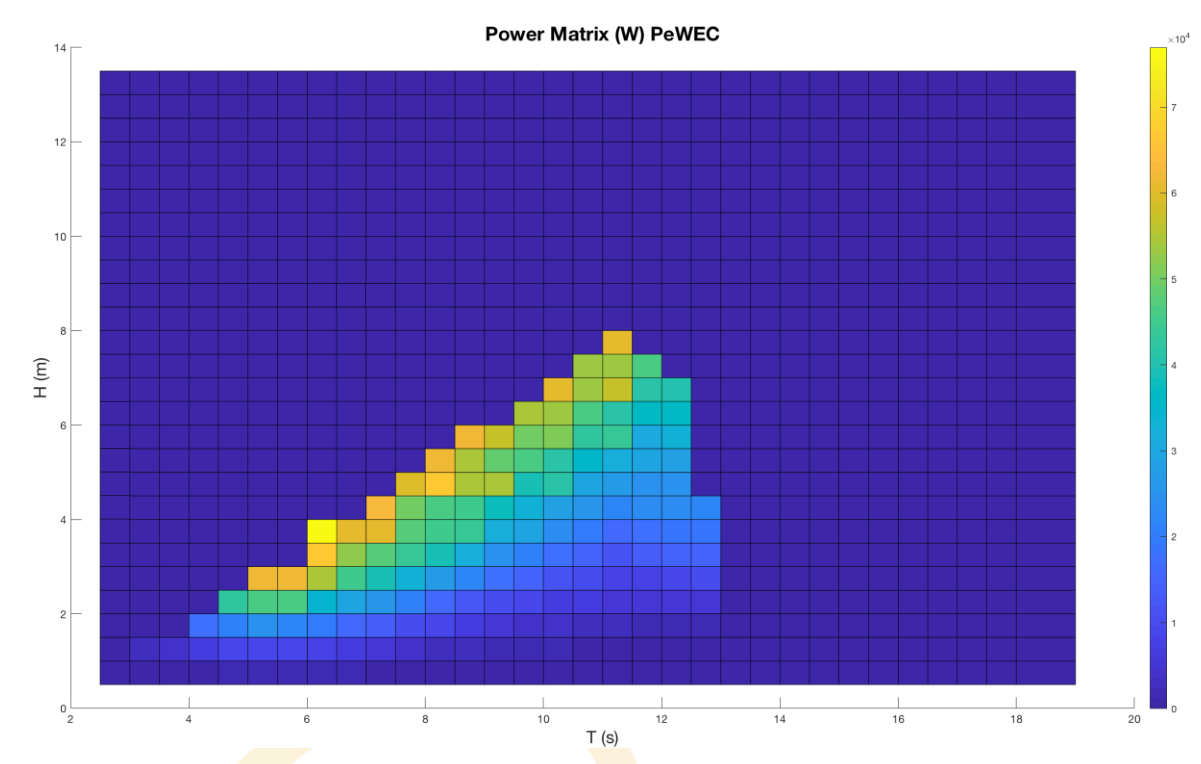
\includegraphics[width=0.8\linewidth]{wec_power_matrix}
	\caption{Matrice di Protenza per la tecnologia WEC}
	\label{fig:wec_power_matrix}
\end{figure}

Tramite la matrice di potenza, quindi, a ogni coppia di valori di $h$ e $T$ è associata la potenza prodotta del dispositivo in una data ora.
Per semplicità non è stato preso in considerazione il parametro della direzione dell'onda. 
Dopo aver ricavato la potenza massima che il dispositivo sarebbe in grado di produrre dalla matrice (valore massimo tra le produttività caratteristiche dei vari stati di mare per quel dato dispositivo) per ogni ora per ottenere il CF si divide la potenza prodotta per la potenza massima:
\begin{equation}
	\text{CF}_\text{WEC} = \frac{M_{hT}}{\text{max}\{M\}}
\end{equation}
Dove $M$ è la matrice di potenza.
La scelta di utilizzare la potenza massima e non quella installata è dovuta al fatto che, a differenza delle altre due tecnologie precedentemente analizzate, nel WEC è possibile che la potenza installata risulti essere di gran lunga più grande di quella prodotta, e, di conseguenza, per non lavorare con valori di CF molto piccoli, si sceglie di rapportare il CF alla potenza massima prodotta anziché a quella installata. 

Una volta calcolati i CF a ogni ora dell'anno per tutte le tecnologie è fondamentale andare a considerare i consumi effettivi delle due isole.
Idealmente sarebbe necessario poter conoscere per ogni ora dell'anno quanta elettricità è stata consumata sull'isola. Tuttavia, questa tipologia di dati è spesso non facile da ottenere in quanto richiede la maggior parte delle volte di interloquire con enti privati, difficilmente propensi a fornirli, sia per ragioni confidenziali, sia per motivi di puro interesse.
Viene quindi utilizzata una curva di consumo standard, che riporta per ogni ora dell'anno un coefficiente normalizzato del consumo dell'isola. Riscalando la curva standard e sfruttando il valore di consumo di energia in un anno dell'isola (ricavato dal bando delle isole Verdi PNRR per Lipari e dal sito STSEE per Wallis) si ottiene una buona approssimazione del consumo ora per ora. 
\begin{figure*}[ht]\centering
	\begin{tikzpicture}
		\begin{axis}[
				yshift = 1cm,
				grid=both,
				axis lines = left,
				xlabel = {Mese},
				ylabel = {Consumo Normalizzato},
				date coordinates in=x,
				date ZERO=2019-01-01,
				table/col sep=comma,
				xticklabel=\month,
				width=17cm,
				height=10cm,
			]
			\addplot[line width = 0.13mm, blue] table [
					x=time,
					y=power,
					col sep=comma,
				] {PlotsData/energy_consumption.csv};
		\end{axis}
	\end{tikzpicture}
	\caption{Curva di consumi normalizzata}
	\label{fig:consumption}
\end{figure*}

Infine, è necessario introdurre ancora un elemento di cruciale importanza nel progetto: gli accumulatori.
Questi, infatti, non solo permettono di conservare l'energia prodotta in eccesso e di restituirla quando necessario, permettendo così alla curva della produttività di approssimare meglio la curva dei consumi, ma sono anche fondamentali per la stabilità della rete.
Come tecnologia si sceglie quella a ioni di litio. 
Di tutti i parametri caratteristici dell'accumulatore, ai fini del nostro modello, vengono presi in
considerazione la capacità massima utilizzabile (espressa in MWh) e l'efficienza.
Per questo ultimo parametro in particolare si fa, per semplicità, solo una distinzione tra le fasi di carica e scarica, senza tuttavia tenere conto del fatto che l'efficienza può variare a seconda della percentuale di carica dell'accumulatore e della potenza che deve essere caricata o fornita. 

Raccogliendo i dati ottenuti, si ricava una tabella dove figurano, supposti noti i valori delle potenze installate per ogni tecnologia e la capacità massima degli accumulatori, i Capacity Factor e le relative potenze prodotte per le singole tecnologie, i consumi, lo stato di carica degli accumulatori e la necessaria produzione di diesel per ogni ora dell'anno.
Da questi, sono poi calcolati i valori caratteristici annuali (medi per quanto riguarda il CF e lo stato di carica e totali per la produzione e il consumo).
Conoscendo i valori della produzione di diesel e del consumo totale è quindi possibile calcolare la penetrazione delle FER in rapporto al totale di energia consumata:
\begin{equation}
	\%_\text{FER} = 100 \cdot \left(1 - \frac{E_{\text{Diesel}}}{E_{\text{Consumata}}}\right)
\end{equation}

A questo punto, per conferire concretezza al modello, è necessario introdurre il fattore costi.
I costi delle singole tecnologie sono calcolati a partire dai CAPEX (Costi capitali di installazione della tecnologia), dagli OPEX (Costo di manutenzione della tecnologia) e dalle produttività nel tempo di vita, tenendo anche conto del discount rate \(r\) (dal momento che i prezzi subiscono variazioni col passare del tempo), in modo da ricavare, per ogni tecnologia, il suo LCOE, valore che fornisce l'informazione sul costo di un kWh di energia consumata.

Di seguito i valori utilizzati per le varie tecnologie e la formula usata per il calcolo dell'LCOE, dove \(E\) è l'energia consumata in un anno, \(n\) il numero di anni di vita attesi della tecnologia, e \(r\) è il discount rate associato alle energie rinnovabili, che per la nostra ricerca è stato stimato al \(\SI{3}{\percent}\):
\begin{equation}
	\text{LCOE} =
		P_\text{inst} \cdot \frac{\frac{\text{CAPEX}}{1+r} + \sum\limits_{t=1}^n \frac{\text{OPEX}}{(1+r)^t}}{\sum\limits_{t=1}^n \frac{E}{(1+r)^t}}
	\label{eq:lcoe}
\end{equation}

Si è preferito il calcolo dell'LCOE rispetto al semplice utilizzo del CAPEX, che dà un'informazione abbastanza valida solo se riferita a scenari di breve termine, in quanto interessati in un'analisi un po' più a lungo termine in cui, a fronte di un valore alto del CAPEX, può anche corrispondere un valore di LCOE non altrettanto elevato essendo il primo ammortizzato negli anni.

Per il WEC, trattandosi di una tecnologia innovativa, e quindi non avendo sufficienti dati sperimentali per avere valori precisi di OPEX, è stata presa, come di valore di riferimento, una percentuale del CAPEX (il \(\SI{3}{\percent}\)).
Per quanto riguarda gli accumulatori invece il costo dipende da due aspetti: la capacità in termini di energia immagazzinata e la capacità in termini di potenza massima. Mentre il primo valore è libero, il secondo può essere calcolato prendendo il valore massimo tra le potenze medie orarie scambiate dall'accumulatore. \\
I valori usati sono come segue\cite{IRENA:RenewPowerGen} \cite{OEE:2030Ocean} \cite{OCT:DevelopmentReport}: \\
\begingroup
\renewcommand{\arraystretch}{1.25}
\begin{table}[H]
	\caption{Valori finanziari}
	\centering
	\begin{tabular}{llc}
		\toprule
		Parametro    & Valore & Unità di misura      \\
		\midrule
		CAPEX Solare & $830$  & $\SI{}{\EUR\per\kW}$ \\
		OPEX Solare  & $13$   & $\SI{}{\EUR\per\kW}$ \\
		CAPEX WEC    & $5750$ & $\SI{}{\EUR\per\kW}$ \\
		OPEX WEC     & $13$   & $\SI{}{\EUR\per\kW}$ \\
		CAPEX Eolico & $2993$ & $\SI{}{\EUR\per\kW}$ \\
		OPEX Eolico  & $172$  & $\SI{}{\EUR\per\kW}$ \\
		\bottomrule
	\end{tabular}
	\label{tab:finparameters}
\end{table}
\endgroup \phantom{a} \\
Giunti a questo punto, l'obiettivo è quello di trovare la combinazione di FER, ognuna col suo profilo di produttività, che permetta nell'insieme di approssimare al meglio la curva dei consumi.
Non si può decidere la curva di produttività di una tecnologia, ma si possono decidere quante e quali tecnologie installare.

\subsection{Ottimizzazione}
Una volta determinate le tecnologie potenzialmente installabili sulle due isole, e stabilito un metodo per stimarne i costi annuali, il prossimo passo è cercare la combinazione di FER ottimale per le isole studiate, in modo da minimiazzare i costi, approssimare al meglio la curva di consumi, e sfruttare al massimo le risorse locali.

Dal punto di vista matematico, è possibile sintetizzare il problema in tale modo: a nostra disposizione abbiamo quattro parametri che descrivono il nostro progetto, ovvero la potenza installata in termini di solare, eolico e WEC; e da questi quattro parametri possiamo ricavare un valore, che rappresenta la bontà del progetto.
Ci sono diversi valori che possono essere scelti come rappresentativi del progetto, ma per questo studio si è scelto il costo annuale stimato di produrre energia per tutta l'isola.
Questo valore sintetizza al meglio le esigenze prima descritte, poiché:
\begin{itemize}
	\item è possibile associare un costo alla produzione di energia non rinnovabile, che non deve essere necessariamente realistico, dal momento che in caso il risultato dell'ottimizzazione preveda una percentuale di FER utilizzata non accettabile, si può aggiungere a questo costo una \textit{carbon tax}, ovvero una tassa artificiale dovuta alla natura non sostenibile del produrre energia tramite fonti non rinnovabili,
	\item usando il costo dell'energia prodotta, e non di quella effettivamente consumata, progetti che sprecano troppa energia (producendone più di quanta ne è necessaria e ne è possibile immagazzinare in ogni dato momento) vengono naturalmente svantaggiati dal dover pagare anche l'energia sprecata,
	\item dal momento che il consumo è valutato per l'intera durata dell'anno, nel caso in cui una tecnologia non risultasse produttiva in un determinato periodo dell'anno, altre tecnologie più produttive in quel momento verrebbero incentivate, anche se non più vantaggiose in media
\end{itemize}
Riassumendo, si vuole trovare il minimo della funzione \\ $f: D \to \mathbb{R}^+$ definita come:
\begin{equation}
	\begin{array}{cl}
		f (P_w, P_e, P_s, E_a) = \\
		\text{LCOE}_r(P_w, P_e, P_s, E_a) \cdot E_\text{prodotta} + C_d \cdot E_d(P_w, P_e, P_s, E_a)
	\end{array}
\end{equation}
dove $\text{LCOE}_r$ è la somma degli LCOE di tutte le tecnologie utilizzate, in funzione delle loro potenze o capacità installate, $E_\text{prodotta}$ è l'energia prodotta da esse, $C_\text{d}$ è il costo del diesel, stimato a Wallis come $\SI{510}{\EUR\per\MWh}$ [CIT] e a Lipari come $\SI{390}{\EUR\per\MWh}$, $E_d$ l'ammontare di energia prodotta dal diesel, e $D$ è l'insieme quadridimensionale, che è il prodotto cartesiano degli intervalli di quanta potenza è potenzialmente installabile di ogni tipologia di energia, e di quanti accumulatori è possibile installare sull'isola, che calcola il costo annuale dell'energia.
A tal scopo, si è impiegato un algoritmo genetico.

\subsubsection{Algoritmo Genetico}
Lo scopo dell'algoritmo è trovare i parametri che minimizzano (o massimizzano) il valore di una data funzione.
Per fare ciò, l'algoritmo esegue 4 diverse fasi: \\
\begin{tikzpicture}[node distance=2cm]
	\node (start) [phase] {Setup};
	\node (survival) [phase, right of=start] {Selezione};
	\node (crossover) [phase, right of=survival] {Crossover};
	\node (mutation) [phase, right of=crossover] {Mutazione};

	\draw [arrow] (start) -- (survival);
	\draw [arrow] (survival) -- (crossover);
	\draw [arrow] (crossover) -- (mutation);
	\draw [arrow] (mutation) |- node[below of=crossover]{} ++(-1,1) -- node{} ++(-3,0) -- (survival);
\end{tikzpicture}

% GA specific commands
\newcommand{\vI}{\vec{I}}

\subsubsection{Setup}
Un insieme di \(n\) tuple ordinate viene inizializzato con valori casuali, uniformi in un sottoinsieme arbitrario di \(D\).
Le singole tuple rappresentano un progetto di prova, e sono chiamate individui \(\vI^{(0)}_i\), mentre l'insieme viene chiamato la popolazione \(P_0\).

\subsubsection{Selezione}
Per ogni individuo della popolazione, ne viene calcolata la funzione \(f\) definita prima, chiamata la funzione di fitness.
Questa funzione rappresenta la bontà del progetto, ed è quella il quale output si vuole minimizzare.
Fatto ciò, si costruisce un nuovo insieme, denominato \(P^s_g\), che conterrà tutti gli individui che passeranno alla prossima generazione.
Per fare ciò, si divide l'insieme \(P_g\) in due, in base alla fitness degli individui: il peggiore \(\SI{50}{\percent}\) degli individui verrà scelto per \(P^s_g\) con probabilità \(p_e\), relativamente bassa, mentre il migliore \(\SI{50}{\percent}\) verrà scelto con probabilità \(p_s\), relativamente alta. 

Queste due probabilità vengono scelte arbitrariamente, e sono parametri della simulazione.
\(p_e\) rappresenta la probabilità che un individuo che non sarebbe in grado di sopravvivere sopravviva, mentre \(p_s\) è la probabilità che un individuo sopravviva.
È necessario rendere queste occorrenze casuali per poter permettere all'algoritmo di non bloccarsi su eventuali minimi locali, e quindi di riuscire correttamente ad approssimare il minimo globale.

\subsubsection{Crossover}
In questa fase, vengono creati nuove tuple, per costruire un terzo insieme \(P^c_g\), di numerosità \(m = n - \#(P^s_g)\).
Per fare ciò, vengono scelte randomicamente \(m\) tuple ordinate di due elementi, presi da \(P^s_g\), e vengono creati nuovi individui, i cui primi due parametri sono presi dal primo elemento della tupla, e gli ultimi due parametri sono presi dal secondo elemento della tupla.
In questo modo, i parametri dei migliori individui della scorsa generazione vengono tramandati alla prossima, in modo da ottenere soluzioni ancora più ottimali.

\subsubsection{Mutazione}
Viene definito il nuovo insieme \(P_{g + 1}\), che sarà il punto di partenza per la prossima iterazione della simulazione.
Questo nuovo insieme contiene tutti gli elementi di \(P^s_g\), e una versione modificata di ogni elemento di \(P^c_g\), nella quale ad ognuno dei parametri di ogni singolo individuo viene aggiunta una componente casuale \(X\), distributa uniformemente nell'insieme \([-M_a, M_a]\).
Questo è il passaggio fondamentale che permette all'algoritmo di ottenere nuove soluzioni migliori delle precedenti: anche se la maggior parte di queste mutazioni non risulterano in miglioramenti, quella piccola percentuale che invece sarà migliore avrà una maggiore possibilità di sopravviere rispetto alle altre, e quindi di tramandare la mutazione positiva alle future generazioni.

\subsubsection{Terminazione dell'algoritmo}
L'algoritmo viene terminato una volta processate \(N\) generazioni, o una volta che, dopo dieci generazioni, la fitness del miglior individuo della popolazione non sia variata di più di un valore \(\varepsilon\) di tolleranza.

\subsubsection{Risultati}
Per le simulazioni, sono stati usati come parametri:
\begin{equation*}
	\begin{array}{ll}
		n = 1000            \\
		N = 5000            \\
		\varepsilon = 0.1   \\
		p_e = 5\%           \\
		p_s = 95\%          \\
		M_a = \SI{100}{\kW} \\
	\end{array}
\end{equation*}
Di seguito viene riportato un esempio di simulazione, utilizzando i dati dell'isola di Lipari, e non imponendo restrizioni su \(D\):

\begin{figure}[ht]\centering
	\begin{tikzpicture}
		\begin{axis}[
				yshift = 1cm,
				grid=both,
				axis lines = left,
				xlabel = {Generazione},
				ylabel = {Fitness},
				table/col sep=comma,
				ymin=2 000 000,%423 786,
				% width=17cm,
				% height=10cm,
			]
			\addplot[line width = 0.50mm, blue] table [
					x=generation,
					y=fitness,
					col sep=comma,
				] {PlotsData/fitness.csv};
		\end{axis}
	\end{tikzpicture}
	\caption{Migliore fitness per generazione}
	\label{fig:fitness}
\end{figure}

\begin{table}[H]
	\caption{Progetto calcolato per Lipari}
	\centering
	\begin{tabular}{llc}
		\toprule
		Tecnologia   & Potenza/Capacità Installata \\
		\midrule
		Solare       & \(\SI{22.88}{\MW}\)         \\
		Eolico       & \(\SI{1.213}{\MW}\)         \\
		WEC          & \(\SI{0.000}{\MW}\)         \\
		Accumulatori & \(\SI{72.26}{\MWh}\)       \\
		% Percentuale di FER & \(\SI{85.36}{\percent}\) \\
		\bottomrule
	\end{tabular}
	\label{tab:unbound_lipari}
\end{table}

\subsubsection{Vantaggi e limitazioni}
Per questo progetto, la scelta di questo algoritmo è motivata dall'elevata dimensionalità del problema.
Tramite questo metodo è possibile ottimizzare problemi molto più velocemente di quanto non si possa fare esplorando interamente lo spazio delle soluzioni, o semplicemente provando manualmente a modificare i parametri fino ad ottenere una soluzione accettabile. 

Un'altro vantaggio è che è semplice tenere conto delle limitazioni ambientali nell'algoritmo: è sufficente fare una prova preliminare per cercare di capire quale sia il tipo di tecnologia più conveniente per il dato problema, valutare la fattibilità del progetto proposto, ed in caso si ritenga il progetto impossibile limitare il parametro non desiderato.
È stato questo il caso dell'isola di Lipari, dove le strette limitazioni paesaggistiche, territoriali e politiche rendono impossibile il progetto preferito dall'algoritmo; ma riducendo lo spazio esplorativo è stato comunque possibile trovare soluzioni alternative.

Uno svantaggio immediato dell'algoritmo è che, per la sua natura randomica, non garantisce un risultato ottimale.
Tuttavia, essendo possibile analizzare a posteriori il risultato è possibile rendersi conto abbastanza facilmente di quale sia l'effettiva qualità del progetto, e dallo studio di questo specifico problema è evidente come questa implementazione, sebbene semplicistica, sia più che sufficente per produrre risultati accettabili.


% Dunque, scelte tutte le tecnologie potenzialmente installabili sulle due isole, dati i valori caratteristici calcolati precedentemente (produzione, consumo, costo), al fine di trovare la migliore combinazione di FER (nello specifico i valori delle potenze installate per ogni tecnologia e la capacità degli accumulatori) è stato usato un algoritmo genetico che ha i seguenti obiettivi:
% \begin{enumerate}
% 	\item massimizzare la potenza prodotta
% 	\item approssimare al meglio la curva dei consumi
% 	\item minimizzare i costi
% \end{enumerate}
% % ** descrizione algoritmo **
% L'algoritmo ha prodotto i seguenti risultati: % ** risultati** 
% Questa soluzione puramente ingegneristica deve tuttavia andare necessariamente incontro ad un'analisi di tipo ecologico, antropologico e legislativo che ne validi i risultati o che metta in evidenza limitazioni e problemi che permettano di ridiscutere il modello in modo da ottenere alla fine la soluzione che garantisce un perfetto bilancio tra i vari fattori in gioco.

% Bibliografia
\phantomsection
\nocite{*}
\printbibliography
% \bibliographystyle{unsrt}

\end{document}
